
\chapter{Registration}

\itkpiccaption[Image Registration Concept]{Image registration is the task of
finding a spatial transform mapping on image into
another.\label{fig:ImageRegistrationConcept}}
\parpic(8cm,3cm)[r]{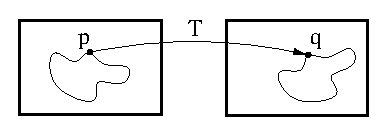
\includegraphics[width=8cm]{ImageRegistrationConcept.eps}}
  
This chapter introduces ITK's capabilities for performing image
registration. Image registration is the process of determining the spatial
transform that maps points from one image to homologous points on a object in
the second image. This concept is schematically represented in Figure
\ref{fig:ImageRegistrationConcept}. In ITK, registration is performed within
a framework of pluggable components that can easily be interchanged.  This
flexibility means that a combinatorial variety of registration methods can be
created, allowing users to pick and choose the right tools for their specific
application.


\section{Registration Framework}
The components of the registration framework and their interconnections 
are shown in Figure \ref{fig:RegistrationComponents}. The basic
input data to the registration process are two images: one
is defined as the \emph{fixed} image $f(\bf{X})$ and the other as the
\emph{moving} image $m(\bf{X})$. Registration is treated as an optimization problem
with the goal of finding the spatial mapping that will bring the moving image into 
alignment with the fixed image.

\begin{figure}
\center
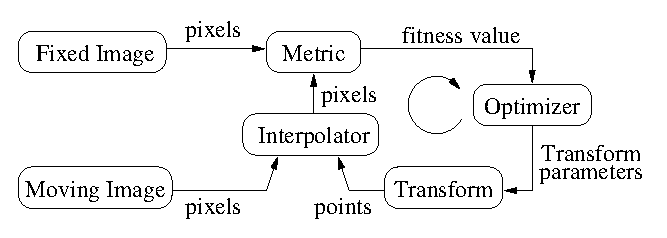
\includegraphics[width=0.8\textwidth]{RegistrationComponentsDiagram.eps}
\itkcaption[Registration Framework Components]{The basic components of the
registration framework are two input images, a transform, a metric, an
interpolator and an optimizer.}
\label{fig:RegistrationComponents}
\end{figure}

The \emph{transform} component $T(\bf{X})$ represents the spatial mapping of
points from the fixed image space to points in the moving image space. Note
that this definition is inverse to the usual view of image transformation.
Using the \emph{inverse} transform is typical in registration as it avoids the
potential problems of ``holes'' with the forward transform. The \emph{interpolator}
is used to evaluate moving image intensity at non-grid positions. The
\emph{metric} component $S(f,m \circ T)$ provides a measure of how well the
fixed image is matched by the transformed moving image. This measure forms the
quantitative criterion to be optimized by the \emph{optimizer} over the search
space defined by the parameters of the \emph{transform}.

These various ITK registration components will be described in later
sections.  First, we begin with some simple registration examples.

\section{"Hello World" Registration}
\label{sec:IntroductionImageRegistration}
\ifitkFullVersion
\input{ImageRegistration1.tex}
\fi

\section{Registration is done in Physical Space}

\begin{figure}
\center
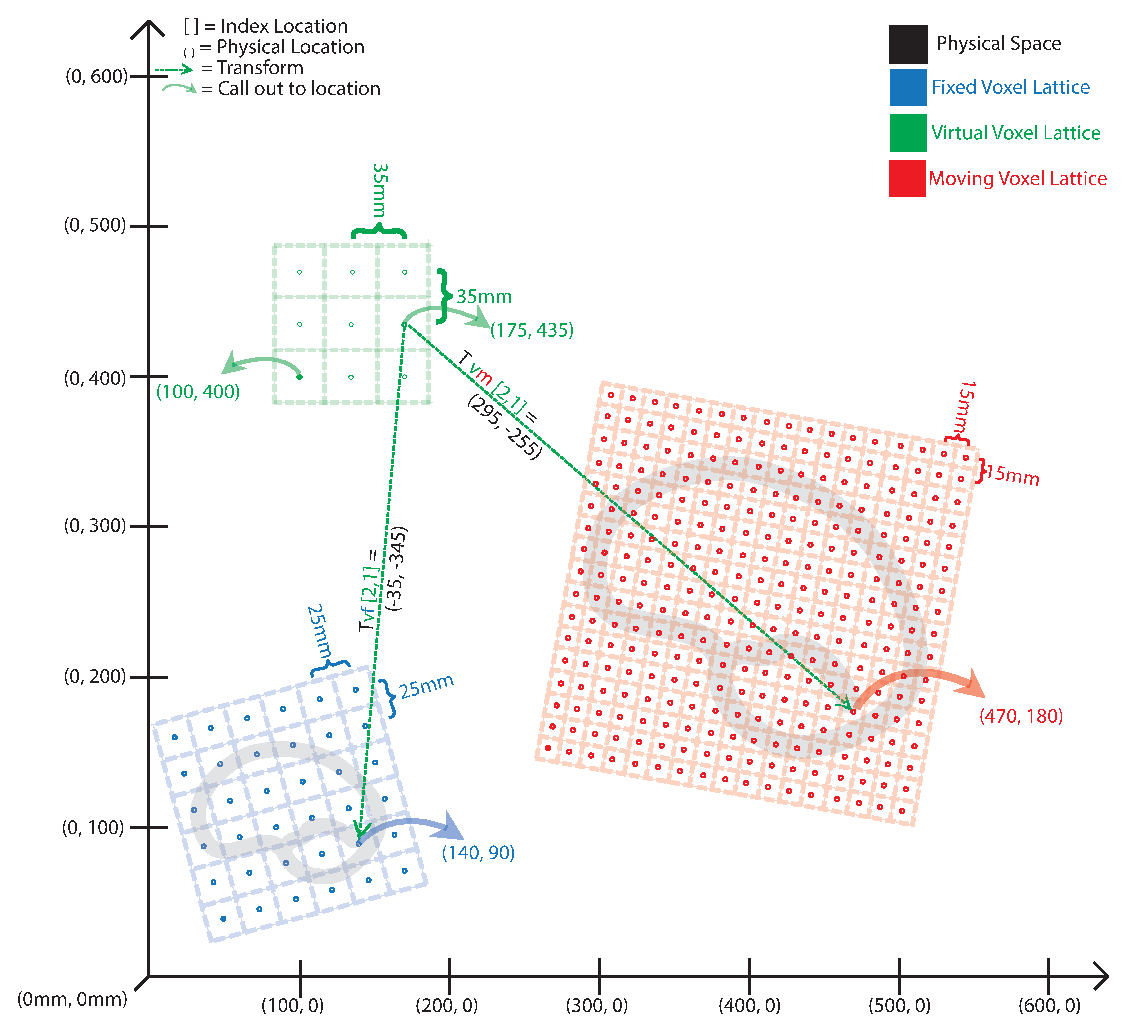
\includegraphics[width=0.8\textwidth]{ImageRegistrationCoordinateSystemsDiagram.eps}
\itkcaption[Registration Coordinate Systems]{Different coordinate systems
involved in the image registration process. Note that the transform being
optimized is the one mapping from the physical space of the fixed image
into the physical space of the moving image.}
\label{fig:ImageRegistrationCoordinateSystemsDiagram}
\end{figure}


This section presents a discussion on the two most common difficulties that
users encounter when they start using the ITK registration framework. They are,
in order of difficulty

\begin{itemize}
\item The direction of the Transform mapping
\item The fact that registration is done in physical coordinates
\end{itemize}

Probably the reason why these two topics tend to create confusion is that they
are implemented in different ways in other systems and therefore users tend to
have a different expectation on how things should work in ITK. The situation
is exacerbated by the fact that most people describe image operations as if
they were manually performed in a picture in paper.

\subsection{Direction of the Transform Mapping}

The Transform that is optimized in the registration framework is the one that
maps points from the physical space of the fixed image into the physical space
of the moving image. This is illustrated in
Figure~\ref{fig:ImageRegistrationCoordinateSystemsDiagram}. This implies that
the Transform will accept as input points from the fixed image and it will
compute the coordinates of the analogous points in the moving image. What tends
to create confusion is the fact that when the Transform shifts a point on the
\textbf{positive} X direction, the visual effect of this mapping, once the
moving image is resampled, is equivalent to {\em manually shifting} the moving
image along the \textbf{negative} X direction. In the same way, when the
Transform applies a \textbf{clock-wise} rotation to the fixed image points, the
visual effect of this mapping once the moving image has been resampled is
equivalent to {\em manually rotating} the moving image
\textbf{counter-clock-wise}. 

The reason why this direction of mapping has been chosen for the ITK
implementation of the registration framework is that this is the direction that
better fits the fact that the moving image is expected to be resampled using
the grid of the fixed image. The nature of the resampling process is such that
an algorithm must go through every pixel of the \textbf{fixed} image and
compute the intensity that should be assigned to this pixel from the mapping of
the moving image. This computation involves to take the integral coordinates of
the pixel in the image grid, usually called the ``(i,j)'' coordinates, map them
into the physical space of the fixed image, then map those physical coordinates
into the physical space of the moving image, then mapping the physical
coordinates of the moving image in to the integral coordinates of the discrete
grid of the moving image, where the value of the pixel intensity will be
computed by interpolation. This sequence of steps is described in
Figure~\ref{fig:ImageRegistrationCoordinateSystemsDiagram}.

If we have used the Transform that maps coordinates from the moving image
physical space into the fixed image physical space, then the resampling process
could not 0 that every pixel in the grid of the fixed image was going
to receive one and only one value. In other words, the resampling will have
resulted in an image with holes and with redundant or overlapped pixel values.

As you have seen in the previous examples, and you will corroborate in the
remaining examples in this chapter, the Transform computed by the registration
framework is the transform that can be used directly in the resampling filter
in order to map the moving image into the grid of the fixed image.

There are exceptional cases in which the transform that you want is actually
the inverse transform of the one computed by the ITK registration framework.
Only in those cases you may have to recur to invoking the \code{GetInverse}
method that most transform offer.  Make sure that before you consider following
that dark path, you interact with the examples of resampling illustrated in
section~\ref{sec:GeometricalTransformationFilters}


\subsection{Registration is done in physical space}

\section{Monitoring Registration}
\label{sec:MonitoringImageRegistration}
\ifitkFullVersion
\input{ImageRegistration3.tex}
\fi



\section{Multi-Modality Registration}
\label{sec:MultiModalityRegistration}

\subsection{Viola-Wells Mutual Information}
\label{sec:MultiModalityRegistrationViolaWells}
\ifitkFullVersion
\input{ImageRegistration2.tex}
\fi

\subsection{Mattes Mutual Information}
\label{sec:MultiModalityRegistrationMattes}
\ifitkFullVersion
\input{ImageRegistration4.tex}
\fi


\subsection{Plotting joint histograms}
\label{sec:JointHistograms}
\ifitkFullVersion
\input{ImageRegistrationHistogramPlotter.tex}


\section{ Centered Transforms }

The ITK image coordinate origin is typically located in one of the image
corners. This results in counter-intuitive transform behavior when
rotations and scaling are involved. Users tend to assume that rotations and
scaling are performed around a fixed point at the center of the image.  In
order to compensate for this difference in natural interpretation, a set of
\emph{centered} transforms have been introduced into the toolkit. The following
sections describe the main characteristics of such transforms.

\subsection{Rigid Registration in 2D}
\label{sec:RigidRegistrationIn2D}
\ifitkFullVersion
\input{ImageRegistration5.tex}
\fi

\subsection{Initializing with Image Moments}
\label{sec:InitializingRegistrationWithMoments}
\ifitkFullVersion
\input{ImageRegistration6.tex}
\fi



%\subsection{Similarity Transform in 2D}
%\label{sec:SimilarityRegistrationIn2D}
%\ifitkFullVersion
%\input{ImageRegistration7.tex}
%\fi



\subsection{Rigid Transform in 3D}
\label{sec:RigidRegistrationIn3D}
\ifitkFullVersion
\input{ImageRegistration8.tex}
\fi




\subsection{Centered Affine Transform}
\label{sec:CenteredAffineTransform}
\ifitkFullVersion
\input{ImageRegistration9.tex}
\fi




\section{Multi-Resolution Registration}
\label{sec:MultiResolutionRegistration}
Performing image registration using a multi-resolution approach is widely used
to improve speed, accuracy and robustness. The basic idea is that registration
is first performed at a coarse scale where the images have fewer pixels.
The spatial mapping determined at the coarse level is then used to initialize
registration at the next finer scale. This process is repeated until it
reaches the finest possible scale. This coarse-to-fine strategy greatly
improve the registration success rate and also increases robustness
by eliminating local optima at coarser scales.

The Insight Toolkit offers a multi-resolution registration framework that is
directly compatible with all the registration framework components. The
multi-resolution registration framework has two additional components: a pair
of \emph{image pyramids} that are used to down-sample the fixed and moving
images as illustrated in Figure \ref{fig:MultiResRegistrationComponents}.
The pyramids smooth and subsample the images according to user-defined
scheduling of shrink factors.
 
\begin{figure}
\center
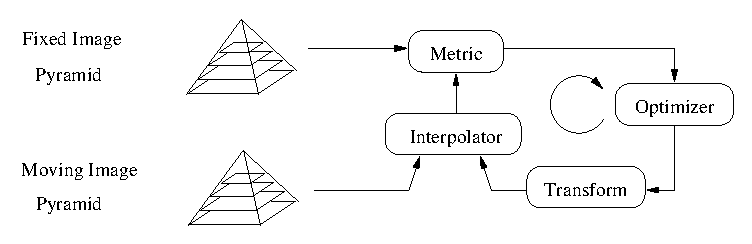
\includegraphics[width=0.8\textwidth]{MultiResRegistrationComponents.eps}
\itkcaption[Multi-Resolution Registration Components]{Components of the
multi-resolution registration framework.}
\label{fig:MultiResRegistrationComponents}
\end{figure}
 
We now present the main capabilities of the multi-resolution framework by
way of an example.

\subsection{Fundamentals}
\ifitkFullVersion
\input{MultiResImageRegistration1.tex}
\fi

\subsection{Parameter Tuning}
\ifitkFullVersion
\input{MultiResImageRegistration2.tex}
\fi

With the completion of these examples, we will now review the main
features of the components forming the registration framework.

\section{Transforms}
\label{sec:Transforms}
\ifitkFullVersion

\def\tableconfiguration{ | p{3cm} | p{1.8cm} | p{2.5cm} | p{4cm} | }


\index{itk::Transform}

\index{Vector!Geometrical Concept}

In the Insight Toolkit, \doxygen{Transform} objects encapsulate the mapping of
points and vectors from an input space to an output space.  If a transform is
invertible, back transform methods are also provided.  Currently, ITK provides
a variety of transforms from simple translation, rotation and scaling to
general affine and kernel transforms.  Note that, while in this section we
discuss transforms in the context of registration, transforms are general and
can be used for other applications. Some of the most commonly used transforms
will be discussed in detail later. Let's begin by introducing the objects used
in ITK for representing basic spatial concepts.


\subsection{Geometrical Representation}
\label{sec:GeometricalObjects}

\begin{figure}
\center
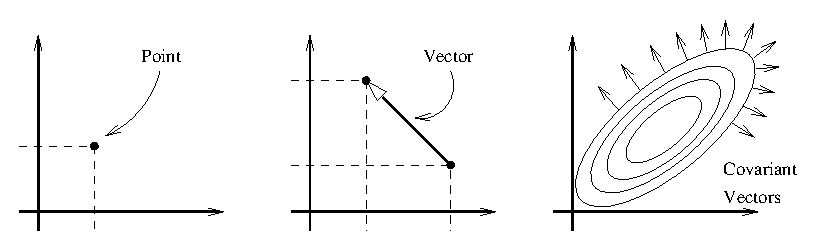
\includegraphics[width=0.9\textwidth]{GeometricalObjects.eps}
\itkcaption[Geometrical representation objects in ITK]{Geometric
representation objects in ITK.}
\label{fig:GeometricalObjects}
\end{figure}
 
ITK implements a consistent geometric representation of the space. The
characteristics of classes involved in this representation are summarized in
Table~\ref{tab:GeometricalConcepts}. In this regard, ITK takes full advantage
of the capabilities of Object Oriented programming and resists the temptation
of using simple arrays of \code{float} or \code{double} in order to represent
geometrical objects. The use of basic arrays would have blurred the important
distinction between the different geometrical concepts and would have allowed
for the innumerable conceptual and programming errors that result from using a
vector where a point is needed or viceversa.

\index{itk::Point!Concept}
\index{itk::Vector!Concept}
\index{itk::CovariantVector!Concept}

\begin{table}
\begin{center}
\begin{tabular}{ | p{0.3\textwidth} | p{ 0.6\textwidth} | }
\hline
\textbf{Class} &
\textbf{Geometrical concept} \\
\hline\hline
\doxygen{Point} & 
Position in space. In $N$-dimensional space it is represented by an array of
$N$ numbers associated with space coordinates. \\
\hline
\doxygen{Vector} & 
Relative position between two points. In $N$-dimensional space it is
represented by an array of $N$ numbers, each one associated with the distance
along a coordinate axis. Vectors do not have a position in space. A vector is
defined as the subtraction of two points.\\
\hline
\doxygen{CovariantVector} & Orthogonal direction to a $(N-1)$-dimensional
manifold in space. For example, in $3D$ it corresponds to the vector orthogonal
to a surface. This is the appropriate class for representing Gradients of
functions. Covariant vectors do not have a position in space. Covariant vector
should not be added to Points, nor to Vectors.\\
\hline
\end{tabular}
\end{center}
\itkcaption[Geometrical Elementary Objects]{Summary of objects representing
geometrical concepts in ITK.\label{tab:GeometricalConcepts}}
\end{table}


Additional uses of the \doxygen{Point}, \doxygen{Vector} and
\doxygen{CovariantVector} classes have been discussed in Chapter
\ref{sec:DataRepresentation}.  Each one of these classes behaves differently
under spatial transformations. It is therefore quite important to keep their
distinction clear. Figure
\ref{fig:GeometricalObjects} illustrates the differences between
these concepts.


\index{itk::Transform!TransformPoint()}
\index{itk::Transform!TransformVector()}
\index{itk::Transform!TransformCovariantVector()}

Transform classes provide different methods for mapping each one of
the basic space-representation objects.  Points, vectors and covariant vectors
are transformed using the methods \code{TransformPoint()},
\code{TransformVector()} and \code{TransformCovariantVector()} respectively.

One of the classes that deserve further comments is the \doxygen{Vector}. This
ITK class tend to be misinterpreted as a container of elements instead of a
geometrical object. This is a common misconception originated by the fact that
Computer Scientist and Software Engineers misuse the term ``Vector''.  The
actual word ``Vector'' is relatively young. It was coined by William Hamilton
in his book ``\emph{Elements of Quaternions}'' published in 1886
(post-mortem)\cite{Hamilton1866}.  In the same text Hamilton coined the terms:
``\emph{Scalar}'', ``\emph{Versor}'' and ``\emph{Tensor}''.  Although the
modern term of ``\emph{Tensor}'' is used in Calculus in a different sense of
what Hamilton defined in his book at the time~\cite{Dodson1997}.

A ``\emph{Vector}'' is, by definition, a mathematical object that embodies the
concept of ``direction in space''. Strictly speaking, a Vector describes the
relationship between two Points in space, and captures both their relative
distance and orientation.

Computer scientists and software engineers missused the term vector in order to
represent the concept of an ``Indexed Set''~\cite{Austern1999}.  Mechanical
Engineers and Civil Engineers, who deal with the real world of physical objects
will not commit this mistake and will keep the word ``\emph{Vector}'' attached
to a geometrical concept.  Biologists, on the other hand, will associate
``\emph{Vector}'' to a ``vehicle'' that allows them to direct something in a
particular direction, for example, a virus that allows them to insert pieces of
code into a DNA strand~\cite{Lodish2000}.

Textbooks in programming do not help to clarify those concepts and losely use
the term ``\emph{Vector}'' for the purpose of representing an ``Enumerated set
of common elements''. STL follows this trend and continue using the word
``\emph{Vector}'' for what it was not supposed to be
used~\cite{Austern1999,Alexandrescu2001}. Linear Algebra devoids the
``\emph{Vector}'' from its notion of Geometrical reality and makes it an
abstract set of numbers with arithmetic operations associated.

For those of you who are looking for the ``\emph{Vector}'' in the Software
Engineering sense, please look at the \doxygen{Array} and \doxygen{FixedArray}
classes that actually provide such functionalities. Additionally, the
\doxygen{VectorContainer} and \doxygen{MapContainer} classes may be of interest
too. These container classes are intended for algorithms that require to insert
and delete elements, and that may have large numbers of elements.

The Insight Toolkit deals with real objects that inhabit the physical space.
This is particularly true in the context of the image registration framework.
We chose to give the appropriate name to the mathematical objects that describe
geometrical relationships in N-Dimensional space. It is for this reason that we
explicitly make clear the distincion between Point, Vector and CovariantVector,
despite the fact that most people would be happy with a simple use of
\code{double[3]} for the three concepts and then will proceed to perform all
sort of conceptually flawed operations such as 

\begin{itemize}
\item Adding two Points
\item Dividing a Point by a Scalar
\item Adding a Covariant Vector to a Point
\item Adding a Covariant Vector to a Vector
\end{itemize}

In order to enforce the correct use of the Geometrical concepts in ITK we
organized these classes in a hierarchy that supports reuse of code and yet
compartamentalize the behavior of the individual classes.  The use of the
\doxygen{FixedArray} as base class of the \doxygen{Point}, the \doxygen{Vector}
and the \doxygen{CovariantVector} was a design decision based on calling things
by their correct name.

An \doxygen{FixedArray} is an enumerated collection with a fixed number of
elements. You can instantiate a fixed array of letters, or a fixed array of
images, or a fixed array of transforms, or a fixed array of geometrical shapes.
Therefore, the FixedArray only implements the functionality that is necesary to
access those enumerated elements. No assumptions can be made at this point on
any other operations required by the elements of the FixedArray, except the
fact of having a default constructor.

The \doxygen{Point} is a type that represents the spatial coordinates of a
spatial location. Based on geometrical concepts we defined the valid operations
of the Point class. In particular we made sure that no \code{operator+()} was
defined between Points, and that no \code{operator*( scalar )} nor
\code{operator/( scalar )} were defined for Points.

In other words, you could do in ITK operations such as:

\begin{itemize}
\item Vector  = Point - Point
\item Point  +=  Vector
\item Point  -=  Vector
\item Point  = BarycentricCombination( Point, Point )
\end{itemize}

and you cannot (because you \textbf{should not}) do operation such as

\begin{itemize}
\item Point = Point * Scalar    
\item Point = Point + Point    
\item Point = Point / Scalar  
\end{itemize}

The \doxygen{Vector} is, by Hamilton's definition, the subtraction between two
points. Therefore a Vector must satisfy the following basic operations:

\begin{itemize}
\item Vector = Point - Point
\item Point  = Point + Vector
\item Point  = Point - Vector
\item Vector = Vector + Vector
\item Vector = Vector - Vector
\end{itemize}

An \doxygen{Vector} object is intended to be instantiated over elements that
support matematical operation such as addition, subtraction and multiplication
by scalars.


\subsection{Transform General Properties}
\label{sec:TransformGeneralProperties}

\index{itk::Transform!SetParameters()} Each transform class typically has
several methods for setting its parameters.  For example,
\doxygen{Euler2DTransform} provides methods for specifying the offset,
angle, and the entire rotation matrix.  However, for use in the
registration framework, the parameters are represented by a flat
Array of doubles to facilitate communication with generic
optimizers. In the case of the Euler2DTransform, the transform is also
defined by three doubles: the first representing the angle, and the last two the
offset. The flat array of parameters is defined using \code{SetParameters()}. A
description of the parameters and their ordering is documented in the 
sections that follow.
 
In the context of registration, the transform parameters define the search
space for optimizers. That is, the goal of the optimization is to find the set
of parameters defining a transform that results in the best possible value of
an image metric. The more parameters a transform has, the longer its
computational time will be when used in a registration method since the
dimension of the search space will be equal to the number of transform
parameters.

\index{itk::Transform!GetJacobian()}

Another requirement that the registration framework imposes on the transform
classes is the computation of their Jacobians. In general, metrics require
the knowledge of the Jacobian in order to compute Metric derivatives.
The Jacobian is a matrix whose element are the partial derivatives of the
output point with respect to the array of parameters that defines the
transform:\footnote{Note that the term \emph{Jacobian} is also commonly used
for the matrix representing the derivatives of output point coordinates with
respect to input point coordinates. Sometimes the term is loosely used to
refer to the determinant of such a matrix.~\cite{Dodson1997}}

\begin{equation}
J=\left[ \begin{array}{cccc}
\frac{\partial x_{1}}{\partial p_{1}} & 
\frac{\partial x_{1}}{\partial p_{2}} & 
\cdots  & \frac{\partial x_{1}}{\partial p_{m}}\\
\frac{\partial x_{2}}{\partial p_{1}} & 
\frac{\partial x_{2}}{\partial p_{2}} & 
\cdots  & \frac{\partial x_{2}}{\partial p_{m}}\\
\vdots  & \vdots  & \ddots  & \vdots \\
\frac{\partial x_{n}}{\partial p_{1}} & 
\frac{\partial x_{n}}{\partial p_{2}} & 
\cdots  & \frac{\partial x_{n}}{\partial p_{m}}
\end{array}\right]
\end{equation}

where $\{p_i\}$ are the transform parameters and $\{x_i\}$ are the coordinates
of the output point.  Within this framework, the Jacobian is represented by an
\doxygen{Array2D} of doubles and is obtained from the transform by method
\code{GetJacobian()}. The Jacobian can be interpreted as a matrix that
indicates for a point in the input space how much its mapping on the output
space will change as a response to a small variation in one of the transform
parameters. Note that the values of the Jacobian matrix depend on the point in
the input space. So actually the Jacobian can be noted as $J(\bf{X})$, where
${\bf{X}}=\{x_i\}$. The use of transform Jacobians enables the efficient
computation of metric derivatives.  When Jacobians are not available, metrics
derivatives have to be computed using finite difference at a price of $2M$
evaluations of the metric value, where $M$ is the number of transform
parameters.

The following sections describe the main characteristics of the transform
classes available in ITK.

\subsection{Identity Transform}
\label{sec:IdentityTransform}
\index{itk::IdentityTransform}

\begin{table}
\begin{center}
\begin{tabular}{\tableconfiguration}
\hline
\textbf{Behavior} &
\textbf{Number of Parameters} &
\textbf{Parameter Ordering} &
\textbf{Restrictions} \\
\hline\hline
Maps every point to itself, every vector to itself and every covariant vector to itself.  & 
0 &
NA  &  
Only defined when the input and output space has the same number of dimensions. \\
\hline
\end{tabular}
\end{center}
\itkcaption[Identity Transform Characteristics]{Characteristics of the identity transform.
\label{tab:IdentityTransformCharacteristics}}
\end{table}

The identity transform \doxygen{IdentityTransform} is mainly used for debugging
purposes. It is provided to methods that require a transform and in cases where
we want to have the certainty that the transform will have no effect whatsoever
in the outcome of the process. It is just a \code{NULL} operation. The main
characteristics of the identity transform are summarized in
Table~\ref{tab:IdentityTransformCharacteristics}


\subsection{Translation Transform}
\label{sec:TranslationTransform}
\index{itk::TranslationTransform}

\begin{table}
\begin{center}
\begin{tabular}{\tableconfiguration}
\hline
\textbf{Behavior} &
\textbf{Number of Parameters} &
\textbf{Parameter Ordering} &
\textbf{Restrictions} \\
\hline\hline
Represents a simple translation of points in the input space
and has no effect on vectors or covariant vectors. &
Same as the input space dimension. &
The $i$-th parameter represents the translation in the $i$-th dimension. &
Only defined when the input and output space has the same number of dimensions. \\
\hline
\end{tabular}
\end{center}
\itkcaption[Translation Transform Characteristics]{Characteristics of the TranslationTransform class.
\label{tab:TranslationTransformCharacteristics}}
\end{table}

The \doxygen{TranslationTransform} is probably the simplest yet one of the most
useful transformations.  It maps all Points by adding a Vector to them.  Vector
and covariant vectors remain unchanged under this transformation since they are
not associated with a particular position in space. Translation is the best
transform to use when starting a registration method. Before attempting to
solve for rotations or scaling it is important to overlap the anatomical
objects in both images as much as possible. This is done by resolving the
translational misalignment between the images. Translations also have the
advantage of being fast to compute and having parameters that are easy to
interpret. The main characteristics of the translation transform are presented
in Table~\ref{tab:TranslationTransformCharacteristics}.

\subsection{Scale Transform}
\label{sec:ScaleTransform}
\index{itk::ScaleTransform}

\begin{table}
\begin{center}
\begin{tabular}{\tableconfiguration}
\hline
\textbf{Behavior} &
\textbf{Number of Parameters} &
\textbf{Parameter Ordering} &
\textbf{Restrictions} \\
\hline\hline
Points are transformed by multiplying each one of their coordinates by the
corresponding scale factor for the dimension.  Vectors are transformed as
points.  Covariant vectors are transformed by \emph{dividing} their components
by the scale factor in the corresponding dimension.  &
Same as the input space dimension. &
The $i$-th parameter represents the scaling in the $i$-th dimension. &
Only defined when the input and output space has the same number of dimensions. \\
\hline
\end{tabular}
\end{center}
\itkcaption[Scale Transform Characteristics]{Characteristics of the ScaleTransform class.
\label{tab:ScaleTransformCharacteristics}}
\end{table}

The \doxygen{ScaleTransform} represents a simple scaling of the
vector space.  Different scaling factors can be applied along each
dimension. Points are transformed by multiplying each one of their
coordinates by the corresponding scale factor for the dimension.  Vectors are
transformed in the same way as points.  Covariant vectors, on the other hand,
are transformed differently since anisotropic scaling does not preserve
angles. Covariant vectors are transformed by \emph{dividing} their components
by the scale factor of the corresponding dimension. In this way, if a
covariant vector was orthogonal to a vector, this orthogonality will be
preserved after the transformation. The following equations summarize the
effect of the transform on the basic geometric objects.

\begin{equation}
\begin{array}{lccccccc}
\mbox{Point }          & \bf{P'} &  =  & T(\bf{P})  & : & \bf{P'}_i &  = & \bf{P}_i \cdot S_i \\
\mbox{Vector}          & \bf{V'} &  =  & T(\bf{V})  & : & \bf{V'}_i &  = & \bf{V}_i \cdot S_i \\
\mbox{CovariantVector} & \bf{C'} &  =  & T(\bf{C})  & : & \bf{C'}_i &  = & \bf{C}_i /     S_i \\
\end{array}
\end{equation}

where $\bf{P}_i$, $\bf{V}_i$ and $\bf{C}_i$ are the point, vector and covariant
vector $i$-th components while $\bf{S}_i$ is the scaling factor along dimension
$i-th$.  The following equation illustrates the effect of the scaling transform
on a $3D$ point.

\begin{equation}
\left[ 
\begin{array}{c}
x' \\
y' \\
z' \\
\end{array}
\right]
=
\left[ 
\begin{array}{ccc}
S_1 &  0  &  0  \\
 0  & S_2 &  0  \\
 0  &  0  & S_3 \\
\end{array}
\right]
\cdot
\left[ 
\begin{array}{c}
x  \\
y  \\
z  \\
\end{array}
\right]
\end{equation}

Scaling appears to be a simple transformation but there are actually a
number of issues to keep in mind when using different scale factors along
every dimension. There are subtle effects---for example, when computing image
derivatives. Since derivatives are represented by covariant vectors, their
values are not intuitively modified by scaling transforms.

One of the difficulties with managing scaling transforms in a registration
process is that typical optimizers manage the parameter space as a vector
space where addition is the basic operation. Scaling is better treated in the
frame of a logarithmic space where additions result in regular multiplicative
increments of the scale. Gradient descent optimizers have trouble updating
step length, since the effect of an additive increment on a scale factor
diminishes as the factor grows. In other words, a scale factor variation of
$(1.0+ \epsilon)$ is quite different from a scale variation of
$(5.0+\epsilon)$.

Registrations involving scale transforms require careful monitoring of the
optimizer parameters in order to keep it progressing at a stable pace. Note
that some of the transforms discussed in following sections, for example, the
AffineTransform, have hidden scaling parameters and are therefore
subject to the same vulnerabilities of the ScaleTransform.

In cases involving misalignments with simultaneous translation, rotation and
scaling components it may be desirable to solve for these components
independently. The main characteristics of the scale transform are presented in
Table~\ref{tab:ScaleTransformCharacteristics}.


\subsection{Scale Logarithmic Transform}
\label{sec:ScaleLogarithmicTransform}
\index{itk::ScaleLogarithmicTransform}

\begin{table}
\begin{center}
\begin{tabular}{\tableconfiguration}
\hline
\textbf{Behavior} &
\textbf{Number of Parameters} &
\textbf{Parameter Ordering} &
\textbf{Restrictions} \\
\hline\hline
Points are transformed by multiplying each one of their coordinates by the
corresponding scale factor for the dimension.  Vectors are transformed as
points.  Covariant vectors are transformed by \emph{dividing} their components
by the scale factor in the corresponding dimension. 
&
Same as the input space dimension. &
The $i$-th parameter represents the scaling in the $i$-th dimension. &
Only defined when the input and output space has the same number of dimensions.
The difference between this transform and the ScaleTransform is that here the
scaling factors are passed as logarithms, in this way their behavior is closer
to the one of a Vector space.  \\
\hline
\end{tabular}
\end{center}
\itkcaption[Scale Logarithmic Transform Characteristics]{Characteristics of the ScaleLogarithmicTransform class.
\label{tab:ScaleLogarithmicTransformCharacteristics}}
\end{table}

The \doxygen{ScaleLogarithmicTransform} is a simple variation of the
\doxygen{ScaleTransform}. It is intended to improve the behavior of the scaling
parameters when they are modified by optimizers. The difference between this
transform and the ScaleTransform is that the parameter factors are passed here
as logarithms. In this way, multiplicative variations in the scale become
additive variations in the logarithm of the scaling factors.




\subsection{Euler2DTransform}
\label{sec:Euler2DTransform}
\index{itk::Euler2DTransform}

\begin{table}
\begin{center}
\begin{tabular}{\tableconfiguration}
\hline
\textbf{Behavior} &
\textbf{Number of Parameters} &
\textbf{Parameter Ordering} &
\textbf{Restrictions} \\
\hline\hline
Represents a $2D$ rotation and a $2D$ translation. Note that the translation
component has no effect on the transformation of vectors and covariant vectors. &
3 &
The first parameter is the angle in radians and the last two parameters
are the translation in each dimension. &
Only defined for two-dimensional input and output spaces. \\
\hline
\end{tabular}
\end{center}
\itkcaption[Euler2D Transform Characteristics]{Characteristics of the Euler2DTransform class.
\label{tab:Euler2DTransformCharacteristics}}
\end{table}

\doxygen{Euler2DTransform} implements a rigid transformation in $2D$. It is 
composed of a plane rotation and a two-dimensional translation. The rotation
is applied first, followed by the translation. The following equation
illustrates the effect of this transform on a $2D$ point,


\begin{equation}
\left[ 
\begin{array}{c}
x' \\
y' \\
\end{array}
\right]
=
\left[ 
\begin{array}{cc}
\cos{\theta} & -\sin{\theta} \\
\sin{\theta} &  \cos{\theta} \\
\end{array}
\right]
\cdot
\left[ 
\begin{array}{c}
x  \\
y  \\
\end{array}
\right]
+ 
\left[ 
\begin{array}{c}
T_x  \\
T_y  \\
\end{array}
\right]
\end{equation}

where $\theta$ is the rotation angle and $(T_x,T_y)$ are the components of the
translation.

A challenging aspect of this transformation is the fact that translations and
rotations do not form a vector space and cannot be managed as linear
independent parameters. Typical optimizers make the loose assumption that
parameters exist in a vector space and rely on the step length to be small
enough for this assumption to hold approximately.

In addition to the non-linearity of the parameter space, the most common
difficulty found when using this transform is the difference in units used
for rotations and translations. Rotations are measured in radians; hence,
their values are in the range $[-\pi,\pi]$. Translations are measured in
millimeters and their actual values vary depending on the image modality
being considered. In practice, translations have values on the order of $10$
to $100$. This scale difference between the rotation and translation
parameters is undesirable for gradient descent optimizers because they
deviate from the trajectories of descent and make optimization slower and more
unstable. In order to compensate for these differences, ITK optimizers accept
an array of scale values that are used to normalize the parameter space.

Registrations involving angles and translations should take advantage of the
scale normalization functionality in order to obtain the best performance out
of the optimizers. The main characteristics of the Euler2DTransform class
are presented in Table~\ref{tab:Euler2DTransformCharacteristics}.


\subsection{CenteredRigid2DTransform}
\label{sec:CenteredRigid2DTransform}
\index{itk::CenteredRigid2DTransform}

\begin{table}
\begin{center}
\begin{tabular}{\tableconfiguration}
\hline
\textbf{Behavior} &
\textbf{Number of Parameters} &
\textbf{Parameter Ordering} &
\textbf{Restrictions} \\
\hline\hline
Represents a $2D$ rotation around a user-provided center followed by a $2D$ translation.&
5 &
The first parameter is the angle in radians. Second and third are the center of
rotation coordinates and the last two parameters are the translation in each
dimension. & 
Only defined for two-dimensional input and output spaces. \\
\hline
\end{tabular}
\end{center}
\itkcaption[CenteredRigid2D Transform Characteristics]{Characteristics of the CenteredRigid2DTransform class.
\label{tab:CenteredRigid2DTransformCharacteristics}}
\end{table}

\doxygen{CenteredRigid2DTransform} implements a rigid transformation in $2D$.
The main difference between this transform and the \doxygen{Euler2DTransform}
is that here we can specify an arbitrary center of rotation, while the
Euler2DTransform always uses the origin of the coordinate system as the center
of rotation. This distinction is quite important in image registration since
ITK images usually have their origin in the corner of the image rather than the
middle.  Rotational mis-registrations usually exist, however, as rotations
around the center of the image, or at least as rotations around a point in the
middle of the anatomical structure captured by the image. Using gradient
descent optimizers, it is almost imposible to solve non-origin rotations using
a transform with origin rotations since the deep basin of the real solution is
usually located across a high ridge in the topography of the cost function.

In practice, the user must supply the center of rotation in the input space,
the angle of rotation and a translation to be applied after the rotation. With
these parameters, the transform initializes a rotation matrix and a translation
vector that together perform the equivalent of translating the center of
rotation to the origin of coordinates, rotating by the specified angle,
translating back to the center of rotation and finally translating by the
user-specified vector.

As with the Euler2DTransform, this transform suffers from the difference in
units used for rotations and translations. Rotations are measured in radians;
hence, their values are in the range $[-\pi,\pi]$. The center of rotation and
the translations are measured in millimeters, and their actual values vary
depending on the image modality being considered.  Registrations involving
angles and translations should take advantage of the scale normalization
functionality of the optimizers in order to get the best performance out of
them.

The following equation illustrates the effect of the transform on an input
point $(x,y)$ that maps to the output point $(x',y')$,

\begin{equation}
\left[ 
\begin{array}{c}
x' \\
y' \\
\end{array}
\right]
=
\left[ 
\begin{array}{cc}
\cos{\theta} & -\sin{\theta} \\
\sin{\theta} &  \cos{\theta} \\
\end{array}
\right]
\cdot
\left[ 
\begin{array}{c}
x - C_x \\
y - C_y \\
\end{array}
\right]
+ 
\left[ 
\begin{array}{c}
T_x + C_x \\
T_y + C_y \\
\end{array}
\right]
\end{equation}

where $\theta$ is the rotation angle, $(C_x,C_y)$ are the coordinates of the
rotation center and $(T_x,T_y)$ are the components of the translation. Note
that the center coordinates are subtracted before the rotation and added back
after the rotation. The main features of the CenteredRigid2DTransform are 
presented in Table~\ref{tab:CenteredRigid2DTransformCharacteristics}.


\subsection{Similarity2DTransform}
\label{sec:Similarity2DTransform}
\index{itk::Similarity2DTransform}

\begin{table}
\begin{center}
\begin{tabular}{\tableconfiguration}
\hline
\textbf{Behavior} &
\textbf{Number of Parameters} &
\textbf{Parameter Ordering} &
\textbf{Restrictions} \\
\hline\hline
Represents a $2D$ rotation, homogeneous scaling and a $2D$ translation. Note that
the translation component has no effect on the transformation of vectors and
covariant vectors. & 
4 &
The first parameter is the scaling factor for all dimensions, the second is the
angle in radians, and the last two parameters are the translations in $(x,y)$
respectively. & 
Only defined for two-dimensional input and output spaces. \\
\hline
\end{tabular}
\end{center}
\itkcaption[Similarity2D Transform Characteristics]{Characteristics of the Similarity2DTransform class.
\label{tab:Similarity2DTransformCharacteristics}}
\end{table}

The \doxygen{Similarity2DTransform} can be seen as a rigid transform combined
with an isotropic scaling factor. This transform preserves angles between
lines. In its $2D$ implementation, the four parameters of this transformation
combine the characteristics of the \doxygen{ScaleTransform} and
\doxygen{Euler2DTransform}. In particular, those relating to the non-linearity
of the parameter space and the non-uniformity of the measurement units.
Gradient descent optimizers should be used with caution on such parameter
spaces since the notions of gradient direction and step length are ill-defined.

The following equation illustrates the effect of the transform on an input
point $(x,y)$ that maps to the output point $(x',y')$,

\begin{equation}
\left[ 
\begin{array}{c}
x' \\
y' \\
\end{array}
\right]
=
\left[ 
\begin{array}{cc}
\lambda &    0     \\
   0    &  \lambda \\
\end{array}
\right]
\cdot
\left[ 
\begin{array}{cc}
\cos{\theta} & -\sin{\theta} \\
\sin{\theta} &  \cos{\theta} \\
\end{array}
\right]
\cdot
\left[ 
\begin{array}{c}
x - C_x \\
y - C_y \\
\end{array}
\right]
+ 
\left[ 
\begin{array}{c}
T_x + C_x \\
T_y + C_y \\
\end{array}
\right]
\end{equation}

where $\lambda$ is the scale factor, $\theta$ is the rotation angle,
$(C_x,C_y)$ are the coordinates of the rotation center and $(T_x,T_y)$ are the
components of the translation. Note that the center coordinates are subtracted
before the rotation and scaling, and they are added back afterwards.  The main
features of the Similarity2DTransform are presented in
Table~\ref{tab:Similarity2DTransformCharacteristics}.


A possible approach for controlling optimization in the parameter space of
this transform is to dynamically modify the array of scales passed to the
optimizer. The effect produced by the parameter scaling can be used to steer
the walk in the parameter space (by giving preference to some of the
parameters over others). For example, perform some iterations updating only
the rotation angle, then balance the array of scale factors in the optimizer
and perform another set of iterations updating only the translations.


\subsection{QuaternionRigidTransform}
\label{sec:QuaternionRigidTransform}
\index{itk::QuaternionRigidTransform}

\begin{table}
\begin{center}
\begin{tabular}{| p{4cm} | p{1.8cm} | p{2.5cm} | p{3cm} |}
\hline
\textbf{Behavior} &
\textbf{Number of Parameters} &
\textbf{Parameter Ordering} &
\textbf{Restrictions} \\
\hline\hline
Represents a $3D$ rotation and a $3D$ translation. The rotation is specified as a
quaternion, defined by a set of four numbers $\bf{q}$.  The relationship
between quaternion and rotation about vector $\bf{n}$ by angle $\theta$ is as
follows: \[ \bf{q} = (\bf{n}\sin(\theta/2), \cos(\theta/2))\] Note that if the
quaternion is not of unit length, scaling will also result. &
7 &
The first four parameters defines the quaternion and the last three parameters
the translation in each dimension. &
Only defined for three-dimensional input and output spaces. \\
\hline
\end{tabular}
\end{center}
\itkcaption[QuaternionRigid Transform Characteristics]{Characteristics of the QuaternionRigidTransform class.
\label{tab:QuaternionRigidTransformCharacteristics}}
\end{table}

The \doxygen{QuaternionRigidTransform} class implements a rigid
transformation in $3D$ space. The rotational part of the transform is
represented using a quaternion while the translation is represented with a
vector. Quaternions components do not form a vector space and hence raise the
same concerns as the \doxygen{Similarity2DTransform} when used with gradient
descent optimizers.

The \doxygen{QuaternionRigidTransformGradientDescentOptimizer} was introduced into the toolkit to address these concerns.  This specialized optimizer implements a variation of a
gradient descent algorithm adapted for a quaternion space.  This class
insures that after advancing in any direction on the parameter space, the
resulting set of transform parameters is mapped back into the permissible
set of parameters. In practice, this comes down to normalizing the newly-computed quaternion to make sure that the transformation remains rigid and no
scaling is applied.  The main characteristics of the
QuaternionRigidTransform are presented in
Table~\ref{tab:QuaternionRigidTransformCharacteristics}.

The Quaternion rigid transform also accepts a user-defined center of rotation.
In this way, the transform can easily be used for registering images where the
rotation is mostly relative to the center of the image instead one of the
corners. The coordinates of this rotation center are not subject to
optimization. They only participate in the computation of the mappings for
Points and in the computation of the Jacobian. The transformations for Vectors
and CovariantVector are not affected by the selection of the rotation center.



\subsection{VersorTransform}
\label{sec:VersorTransform}
\index{itk::VersorTransform}
\index{itk::VersorTransformOptimizer}
\index{itk::Versor!Definition}

\begin{table}
\begin{center}
\begin{tabular}{\tableconfiguration}
\hline
\textbf{Behavior} &
\textbf{Number of Parameters} &
\textbf{Parameter Ordering} &
\textbf{Restrictions} \\
\hline\hline
Represents a $3D$ rotation. The rotation is specified by a versor or unit
quaternion. The rotation is performed around a user-specified center of
rotation.&
3 &
The three parameters define the versor.&
Only defined for three-dimensional input and output spaces. \\
\hline
\end{tabular}
\end{center}
\itkcaption[Versor Transform Characteristics]{Characteristics of the Versor Transform
\label{tab:VersorTransformCharacteristics}}
\end{table}


By definition, a \emph{Versor} is the rotational part of a Quaternion. It can
also be defined as a \emph{unit-quaternion} \cite{Hamilton1866,Joly1905}.
Versors only have three independent components, since they are restricted to
reside in the space of unit-quaternions. The implementation of versors in the
toolkit uses a set of three numbers.  These three numbers correspond to the
first three components of a quaternion.  The fourth component of the quaternion
is computed internally such that the quaternion is of unit length. The main
characteristics of the \doxygen{VersorTransform} are presented in
Table~\ref{tab:VersorTransformCharacteristics}.

This transform exclusively represents rotations in $3D$. It is intended to
rapidly solve the rotational component of a more general misalignment.  The
efficiency of this transform comes from using a parameter space of reduced
dimensionality. Versors are the best possible representation for rotations in
$3D$ space. Sequences of versors allow the creation of smooth rotational
trajectories; for this reason, they behave stably under optimization methods.

The space formed by versor parameters is not a vector space. Standard gradient
descent algorithms are not appropriate for exploring this parameter space. An
optimizer specialized for the versor space is available in the toolkit under
the name of \doxygen{VersorTransformOptimizer}. This optimizer implements
versor derivatives as originally defined by Hamilton \cite{Hamilton1866}.

The center of rotation can be especified by the user with the
\code{SetCenter()} method. The center is not part of the parameters to be
optimized, therefore it remains the same during an optimization process. Its
value is used during the computations for transforming Points and when
computing the Jacobian.

\subsection{VersorRigid3DTransform}
\label{sec:VersorRigid3DTransform}
\index{itk::VersorRigid3DTransform}

\begin{table}
\begin{center}
\begin{tabular}{\tableconfiguration}
\hline
\textbf{Behavior} &
\textbf{Number of Parameters} &
\textbf{Parameter Ordering} &
\textbf{Restrictions} \\
\hline\hline
Represents a $3D$ rotation and a $3D$ translation. The rotation is specified by
a versor or unit quaternion, while the translation is represented by a vector.
Users can specify the coordinates of the center of rotation. &
6 &
The first three parameters define the versor and the last three parameters the
translation in each dimension. &
Only defined for three-dimensional input and output spaces. \\
\hline
\end{tabular}
\end{center}
\itkcaption[Versor Rigid3D Transform Characteristics]{Characteristics of the VersorRigid3DTransform class.
\label{tab:VersorRigid3DTransformCharacteristics}}
\end{table}

The \doxygen{VersorRigid3DTransform} implements a rigid transformation in $3D$
space. It is a variant of the \doxygen{QuaternionRigidTransform} and the
\doxygen{VersorTransform}. It can be seen as a \doxygen{VersorTransform} plus a
translation defined by a vector. The advantage of this class with respect to
the QuaternionRigidTransform is that it exposes only six parameters, three for
the versor components and three for the translational components. This reduces
the search space for the optimizer to six dimensions instead of the seven
dimensional used by the QuaternionRigidTransform.  This transform also allows
the users to set a specific center of rotation. The center coodinates are not
modified during the optimization performed in a registration process.  The main
features of this transform are summarized in
Table~\ref{tab:VersorRigid3DTransformCharacteristics}.  This transform is
probably the best option to use when dealing with rigid transformations in
$3D$. 

Given that the space of Versors is not a Vector space, typical gradient descent
optimizers are not well suited for exploring the parametric space of this
transform. The \doxygen{VersorRigid3DTranformOptimizer} has been
introduced in the ITK toolkit with the purpose of providing an optimizer that
is aware of the Versor space properties on the rotational part of this
transform, as well as the Vector space properties on the translational part of
the transform.


\subsection{Euler3DTransform}
\label{sec:Euler3DTransform}
\index{itk::Euler3DTransform}

\begin{table}
\begin{center}
\begin{tabular}{\tableconfiguration}
\hline
\textbf{Behavior} &
\textbf{Number of Parameters} &
\textbf{Parameter Ordering} &
\textbf{Restrictions} \\
\hline\hline
Represents a rigid rotation in $3D$ space. That is, a rotation followed by a
$3D$ translation. The rotation is specified by three angles representing
rotations to be applied around the X, Y and Z axis one after another.  The
translation part is represented by a Vector. Users can also specify the
coordinates of the center of rotation. &
6 &
The first three parameters are the rotation angles around X, Y and Z axis, and
the last three parameters are the translations along each dimension. &
Only defined for three-dimensional input and output spaces. \\
\hline
\end{tabular}
\end{center}
\itkcaption[Euler3D Transform Characteristics]{Characteristics of the Euler3DTransform class.
\label{tab:Euler3DTransformCharacteristics}}
\end{table}

The \doxygen{Euler3DTransform} implements a rigid transformation in $3D$ space.
It can be seen as a rotation followed by a translation. This class exposes six
parameters, three for the Euler angles that represent the rotation and three
for the translational components. This transform also allows the users to set a
specific center of rotation. The center coodinates are not modified during the
optimization performed in a registration process. The main features of this
transform are summarized in Table~\ref{tab:Euler3DTransformCharacteristics}.  

The fact that the three rotational parameters are non-linears and do not behave
like Vector spaces must be taken into account when selecting an optimizer to
work with this transform and when fine tunning the parameters of such
optimizer. It is strongly recommended to use this transform by introducing very
small variations on the rotaional components. A small rotation will be in the
range of 1 degree, which in radians is approximately $0.0.1745$.

You should not expect this transform to be able to compensate for large
rotations just by being driven with the optimizer. In practice you must provide
a reasonable initialization of the transform angles and only need to correct
for residual rotations in the order of $10$ or $20$ degrees.


\subsection{Similarity3DTransform}
\label{sec:Similarity3DTransform}
\index{itk::Similarity3DTransform}

\begin{table}
\begin{center}
\begin{tabular}{\tableconfiguration}
\hline
\textbf{Behavior} &
\textbf{Number of Parameters} &
\textbf{Parameter Ordering} &
\textbf{Restrictions} \\
\hline\hline
Represents a $3D$ rotation, a $3D$ translation and homogeneous scaling. The
scaling factor is specified by a scalar, the rotation is specified by a versor,
and the translation is represented by a vector.  Users can also specify the
coordinates of the center of rotation, that is the same center used for
scaling. &
7 &
The first parameter is the scaling factor, the next three parameters define the
versor and the last three parameters the translation in each dimension. &
Only defined for three-dimensional input and output spaces. \\
\hline
\end{tabular}
\end{center}
\itkcaption[Similarity3D Transform Characteristics]{Characteristics of the Similarity3DTransform class.
\label{tab:Similarity3DTransformCharacteristics}}
\end{table}

The \doxygen{Similarity3DTransform} implements a similarity transformation in
$3D$ space. It can be seen as an homogeneous scaling followed by a
\doxygen{VersorRigid3DTransform}. This class exposes seven parameters, one for
the scaling factor, three for the versor components and three for the
translational components. This transform also allows the users to set a
specific center of rotation. The center coodinates are not modified during the
optimization performed in a registration process.  Both the rotation and
scaling operations are performed with respect to the center of rotation. The
main features of this transform are summarized in
Table~\ref{tab:Similarity3DTransformCharacteristics}.  

The fact that the scaling and rotational spaces are non-linears and do not
behave like Vector spaces must be taken into account when selecting an
optimizer to work with this transform and when fine tunning the parameters of
such optimizer.


\subsection{Rigid3DPerspectiveTransform}
\label{sec:Rigid3DPerspectiveTransform}
\index{itk::Rigid3DPerspectiveTransform}

\begin{table}
\begin{center}
\begin{tabular}{\tableconfiguration}
\hline
\textbf{Behavior} &
\textbf{Number of Parameters} &
\textbf{Parameter Ordering} &
\textbf{Restrictions} \\
\hline\hline 
Represents a rigid $3D$ transformation followed by a perspective projection.
The rotation is specified by a Versor, while the translation is represented by
a Vector.  Users can specify the coordinates of the center of rotation. They
must specifiy a focal distance to be used for the perspective projection. The
rotation center and the focal distance parameters are not modified during the
optimization process. &
6 &
The first three parameters define the Versor and the last three parameters the
Translation in each dimension. &
Only defined for three-dimensional input and two-dimensional output spaces.
This is one of the few transforms where the input space has a different
dimension from the output space.\\
\hline
\end{tabular}
\end{center}
\itkcaption[Rigid3DPerspective Transform Characteristics]{Characteristics of
the Rigid3DPerspectiveTransform class.
\label{tab:VersorRigid3DTransformCharacteristics}}
\end{table}

The \doxygen{Rigid3DPerspectiveTransform} implements a rigid transformation in
$3D$ space followed by a perspective projection. This transform is intended to
be used in $3D/2D$ registration problems where a 3D object is projected onto a
2D plane. This is the case of Fluoroscopic images used for image guided
intervention, and it is also the case for classical radiography.  Users must
provide a value for the focal distance to be used during the computation of the
perspective transform. This transform also allows users to set a specific
center of rotation. The center coodinates are not modified during the
optimization performed in a registration process.  The main features of this
transform are summarized in
Table~\ref{tab:VersorRigid3DTransformCharacteristics}.  This transform is also
used when creating Digitally Reconstructed Radiographs (DRRs).

The strategies for optimizing the parameters of this transform are the same
ones used for optimizing the VersorRigid3DTransform. In particular, you can use
the same Versor\-Rigid3D\-Tranform\-Optimizer in order to optimize the
parameters of this class.


\subsection{AffineTransform}
\label{sec:AffineTransform}
\index{itk::AffineTransform}

\begin{table}
\begin{center}
\begin{tabular}{\tableconfiguration}
\hline
\textbf{Behavior} &
\textbf{Number of Parameters} &
\textbf{Parameter Ordering} &
\textbf{Restrictions} \\
\hline\hline
Represents an affine transform composed of rotation, scaling, shearing and
translation. The transform is specified by a $N \times N$ matrix and a $N
\times 1$ vector where $N$ is the space dimension. &
$(N+1) \times N$ &
The first $N \times N$ parameters define the matrix in column-major order
(where the column index varies the fastest).  The last $N$ parameters define
the translations for each dimension. &
Only defined when the input and output space have the same dimension. \\
\hline
\end{tabular}
\end{center}
\itkcaption[Affine Transform Characteristics]{Characteristics of the AffineTransform class.
\label{tab:AffineTransformCharacteristics}}
\end{table}

The \doxygen{AffineTransform} is one of the most popular transformations used
for image registration. Its main advantage comes from the fact that it is 
represented as a linear transformation. The main features of this
transform are presented in Table~\ref{tab:AffineTransformCharacteristics}.

The set of AffineTransform coefficients can actually be represented in a vector
space of dimension $(N+1) \times N$. This makes it possible for optimizers to
be used appropriately on this search space. However, the high dimensionality of
the search space also implies a high computational complexity of cost-function
derivatives. The best compromise in the reduction of this computational time is
to use the transform's Jacobian in combination with the image gradient for
computing the cost-function derivatives.

The coefficients of the $N \times N$ matrix can represent rotations,
anisotropic scaling and shearing. These coefficients are usually of a very
different dynamic range compared to the translation
coefficients. Coefficients in the matrix tend to be in the range $[-1:1]$, but
are not restricted to this interval.  Translation coefficients, on the other
hand, can be on the order of $10$ to $100$, and are basically related to the
image size and pixel spacing.

This difference in scale makes it necessary to take advantage of the
functionality offered by the optimizers for rescaling the parameter space. This
is particularly relevant for optimizers based on gradient descent approaches.

A registration based on the affine transform may be more effective when
applied after simpler transformations have been used to remove the major
components of misalignment. Otherwise it will incur an overwhelming
computational cost. For example, using an affine transform, the first set of
optimization iterations would typically focus on removing large
translations. This task could instead be accomplished by a translation
transform in a parameter space of size $N$ instead of the $(N+1) \times N$
associated with the affine transform.

Tracking the evolution of a registration process that uses
AffineTransforms can be challenging, since it is difficult to
represent the coefficients in a meaningful way.  A simple printout of the
transform coefficients generally does not offer a clear picture of the current
behavior and trend of the optimization.  A better implementation uses
the affine transform to deform wire-frame cube which is shown in a $3D$
visualization display.



\subsection{BSplineDeformableTransform}
\label{sec:BSplineDeformableTransform}
\index{itk::BSplineDeformableTransform}

\begin{table}
\begin{center}
\begin{tabular}{\tableconfiguration}
\hline
\textbf{Behavior} &
\textbf{Number of Parameters} &
\textbf{Parameter Ordering} &
\textbf{Restrictions} \\
\hline\hline
Represents a free from deformation by providing a deformation field from the
interpolation of deformations in a coarse grid. 
&
$M \times N$ &
Where $M$ is the number of nodes in the BSpline grid and $N$ is the dimension of the space. &
Only defined when the input and output space have the same dimension. This
transform has the advantage of allowing to compute deformable registration. It
also has the disadvantge of having a very high dimensional parametric space,
and therefore requiring long computation times.\\
\hline
\end{tabular}
\end{center}
\itkcaption[BSpline Deformable Transform Characteristics]{Characteristics of the BSplineDeformableTransform class.
\label{tab:BSplineDeformableTransformCharacteristics}}
\end{table}

The \doxygen{BSplineDeformableTransform} is designed to be used for solving
deformable registration problems. This transform is equivalent to generation a
deformation field where a deformation vector is assigned to every point in
space.  The deformation vectors are computed using BSpline interpolation from
the deformation values of points located in a coarse grid, that is usually
refered to as the BSpline grid.

The BSplineDeformableTransform is not flexible enough for accounting for large
rotations or shearing, or scaling differences. In order to compensate for this
limitation, it provides the functionality of being composed with an arbitrary
transform. This transform is known as the \emph{Bulk} transform and it is
applied to points before they are mapped with the displacement field.

This transform do not provide funcionalities for maping Vectors nor
CovariantVectors, only Points can be mapped. The reason is that the variations
of a vector under a deformable transform actually depend on the location of the
vector in space. In other words, Vector only make sense as the relative
position between two points.

The BSplineDeformableTransform has a very large number of parameters and
therefore is well suited for the \doxygen{LBFGSOptimizer} and
\doxygen{LBFGSBOptimizer}. The use of this transform for was proposed in the
following papers~\cite{Rueckert1999,Mattes2001,Mattes2003}.




\subsection{KernelTransforms}
\label{sec:KernelTransforms}
\index{itk::KernelTransforms}

Kernel Transforms are a set of Transforms that are also suitable for performing
deformable registration. These transforms compute on the fly the displacements
corresponding to a deformation field. The displacement values corresponding to
every point in space are computed by interpolation from the vectors defined by
a set of \emph{Source Landmarks} and a set of \emph{Target Landmarks}.

Several variations of these transforms are available in the toolkit. They
differ on the type of interpolation kernel that is used when computing the
deformation in a particular point of space. Note that these transforms are
computationaly expensive and that they computational complexity is proportional
to the number of landmarks and the space dimension.

The following is the list of Transforms based on the KernelTransform.

\begin{itemize}
\item \doxygen{ElasticBodySplineKernelTransform}
\item \doxygen{ElasticBodyReciprocalSplineKernelTransform}
\item \doxygen{ThinPlateSplineKernelTransform}
\item \doxygen{ThinPlateR2LogRSplineKernelTransform}
\item \doxygen{VolumeSplineKernelTransform}
\end{itemize}

Details about the mathematical background of these transform can be found in
the paper by Davis \emph{et. al}~\cite{Davis1997} and the papers by Rohr
\emph{et. al}~\cite{Rohr1999,Rohr2001}.



\fi



% the clearpage command helps to avoid orphans in the title of the next
% section.
\clearpage

\section{Interpolators}
\label{sec:Interpolators}
\ifitkFullVersion
%
%  This file is included by Registration.tex
%

\begin{figure}
\centering
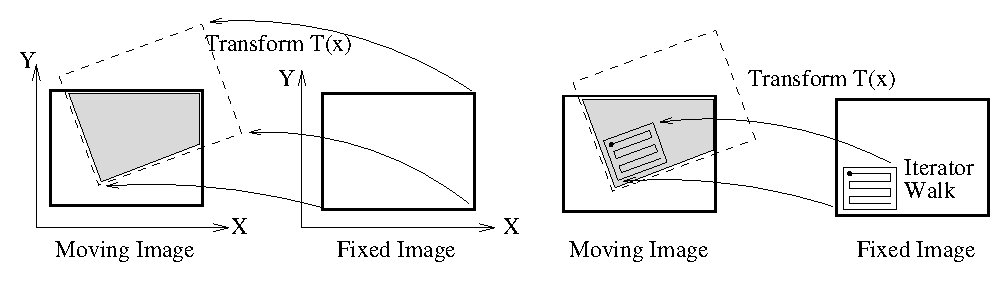
\includegraphics[width=\textwidth]{ImageOverlap.eps}
\itkcaption[Mapping moving image to fixed image in Registration]{ The moving
image is mapped into the fixed image space under some spatial
transformation. An iterator walks through the fixed image and its coordinates
are mapped onto the moving image.}
\label{fig:ImageOverlapIterator}
\end{figure}


\begin{floatingfigure}[rlp]{0.5\textwidth}
 \centering
 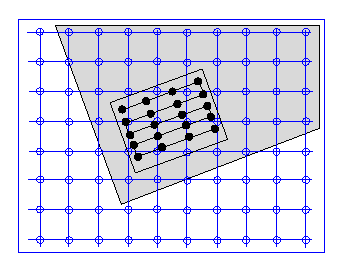
\includegraphics[width=7.5cm]{ImageOverlapInterpolator.eps}
 \caption[Need for interpolation in Registration]{Grid positions of the fixed
image map to non-grid positions of the moving
image.  \label{fig:ImageOverlapInterpolator}}
\end{floatingfigure}

In the registration process, the metric typically compares intensity values
in the fixed image against the corresponding values in the transformed moving
image. When a point is mapped from one space to another by a transform, it
will in general be mapped to a non-grid position. Therefore, interpolation is
required to evaluate the image intensity at the mapped position.

Figure \ref{fig:ImageOverlapIterator} (left) illustrates the mapping of the
fixed image space onto the moving image space. The transform maps points from
the fixed image coordinate system onto the moving image coordinate system. The
figure highlights the region of overlap between the two images after the
mapping. The right side illustrates how an iterator is used to walk through a
region of the fixed image. Each one of the iterator positions is mapped by the
transform onto the moving image space in order to find the homologous pixel.

Figure \ref{fig:ImageOverlapInterpolator} presents a detailed view of the
mapping from the fixed image to the moving image. In general, the grid
positions of the fixed image will not be mapped onto grid positions of the
moving image.  Interpolation is needed for estimating the intensity of the
moving image at these non-grid positions. The service is provided in ITK by
interpolator classes that can be plugged into the registration method.

\index{Nearest\-Neighbor\-Interpolate\-Image\-Function}
\index{Linear\-Interpolate\-Image\-Function}
\index{BSpline\-Interpolate\-Image\-Function}
\index{Windowed\-Sinc\-Interpolate\-Image\-Function}

The following interpolators are available:

\begin{itemize}
\item \doxygen{NearestNeighborInterpolateImageFunction}
\item \doxygen{LinearInterpolateImageFunction}
\item \doxygen{BSplineInterpolateImageFunction}
\item \doxygen{WindowedSincInterpolateImageFunction}
\end{itemize}

In the context of registration, the interpolation method affects the smoothness
of the optimization search space and the overall computation time. On the other
hand, interpolations are executed thousands of times in a single optimization
cycle. Hence, the user has to balance the simplicity of computation with the
smoothness of the optimization when selecting the interpolation scheme.

\index{itk::InterpolateImageFunction}
\index{itk::InterpolateImageFunction!SetInputImage()}
\index{itk::InterpolateImageFunction!Evaluate()}
\index{itk::InterpolateImageFunction!EvaluateAtContinuousIndex()}
\index{itk::InterpolateImageFunction!IsInsideBuffer()}

The basic input to an \doxygen{InterpolateImageFunction} is the image to
be interpolated. Once an image has been defined using \code{SetInputImage()},
a user can interpolate either at a point using \code{Evaluate()} or
an index using \code{EvaluateAtContinuousIndex()}.

Interpolators provide the method \code{IsInsideBuffer()} that tests whether a
particular image index or a physical point falls inside the spatial domain for
which image pixels exist.

\subsection{Nearest Neighbor Interpolation}
\label{sec:NearestNeighborInterpolation}
\index{itk::Nearest\-Neighbor\-Interpolate\-Image\-Function}
The \doxygen{NearestNeighborInterpolateImageFunction} simply uses the
intensity of the nearest grid position. That is, it assumes that the image
intensity is piecewise constant with jumps mid-way between grid positions.
This interpolation scheme is cheap as it does not require any floating point
computations.


\subsection{Linear Interpolation}
\label{sec:LinearInterpolation}
\index{itk::Linear\-Interpolate\-Image\-Function}

The \doxygen{LinearInterpolateImageFunction} assumes that intensity varies
linearly between grid positions. Unlike nearest neighbor interpolation, the
interpolated intensity is spatially continuous. However, the intensity
gradient will be discontinuous at grid positions.


\subsection{B-Spline Interpolation}
\label{sec:BSplineInterpolation}
\index{itk::BSpline\-Interpolate\-Image\-Function}

\begin{figure}
\center
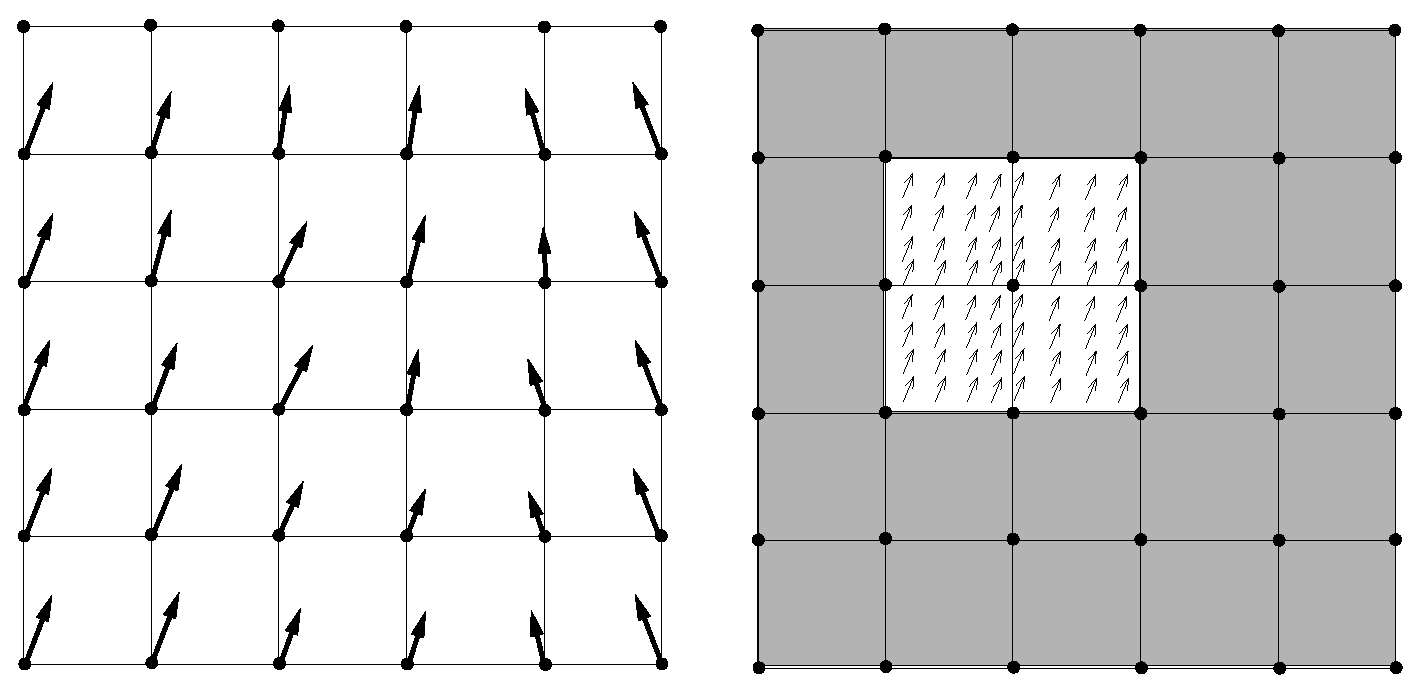
\includegraphics[width=0.9\textwidth]{BSplineInterpolation.eps}
\itkcaption[BSpline Interpolation Concepts]{The left side illustrates the
BSpline grid and the deformations that are known on those nodes. The right side
illustrates the region where interpolation is possible when the BSpline is of
cubic order. The small arrows represent deformation values that were
interpolated from the grid deformations shown on the left side of the diagram.}
\label{fig:BSplineInterpolation}
\end{figure}


The \doxygen{BSplineInterpolateImageFunction} represents the image intensity
using B-spline basis functions. When an input image is first connected to the
interpolator, B-spline coefficients are computed using recursive filtering
(assuming mirror boundary conditions). Intensity at a non-grid position is
computed by multiplying the B-spline coefficients with shifted B-spline kernels
within a small support region of the requested position.
Figure~\ref{fig:BSplineInterpolation} illustrates on the left how the
deformation values on the BSpline grid nodes are used for computing
interpolated deformations in the rest of space. Note for example that when a
cubic BSpline is used, the grid must have one extra node in one side of the
image and two extra nodes on the other side, this along every dimension.

Currently, this interpolator supports splines of order $0$ to $5$. Using a
spline of order $0$ is almost identical to nearest neighbor interpolation; a
spline of order $1$ is exactly identical to linear interpolation. For splines
of order greater than $1$, both the interpolated value and its derivative are
spatially continuous.

It is important to note that when using this scheme, the interpolated
value may lie outside the range of input image intensities. This is
especially important when handling unsigned data, as it is possible
that the interpolated value is negative.


\subsection{Windowed Sinc Interpolation}
\label{sec:WindowedSincInterpolation}
\index{itk::Windowed\-Sinc\-Interpolate\-Image\-Function}

The \doxygen{WindowedSincInterpolateImageFunction} is the best possible
interpolator for data that have been digitized in a discrete grid. This
interpolator has been developed based on Fourier Analysis considerations. It
is well known in signal processing that the process of sampling a spatial
function using a periodic discrete grid results in a replication of the
spectrum of that signal in the frequency domain.

The process of recovering the continuous signal from the discrete sampling is
equivalent to the removal of the replicated spectra in the frequency domain.
This can be done by multiplying the spectra with a box function that will set
to zero all the frequencies above the highest frequency in the original signal.
Multiplying the spectrum with a box function is equivalent to convolving the
spatial discrete signal with a sinc function

\begin{equation}
sinc(x) = \sin{(x)} / x
\end{equation}

The sinc function has infinite support, which of course in practice can not
really be implemented. Therefore, the sinc is usually truncated by multiplying
it with a Window function. The Windowed Sinc interpolator is the result of such an
operation.

This interpolator presents a series of trade-offs in its utilization. Probably
the most significant is that the larger the window, the more precise will be
the resulting interpolation. However, large windows will also result in long
computation times. Since the user can select the window size in this
interpolator, it is up to the user to determine how much interpolation quality
is required in her/his application and how much computation time can be
justified. For details on the signal processing theory behind this
interpolator, please refer to Meijering \emph{et.
al}~\cite{SignalReconstruction}.

The region of the image used for computing the interpolator is determined by
the window \emph{radius}. For example, in a $2D$ image where we want to
interpolate the value at position $(x,y)$ the following computation will be
performed.

\begin{equation}
I(x,y) =
\sum_{i = \lfloor x \rfloor + 1 - m}^{\lfloor x \rfloor + m}
\sum_{j = \lfloor y \rfloor + 1 - m}^{\lfloor y \rfloor + m}
I_{i,j} K(x-i) K(y-j)
\end{equation}

where $m$ is the \emph{radius} of the window. Typically, values such as 3 or 4
are reasonable for the window radius. The function kernel $K(t)$ is composed by
the $sinc$ function and one of the windows listed above.

\begin{equation}
K(t) = w(t) \textrm{sinc}(t) = w(t) \frac{\sin(\pi t)}{\pi t}
\end{equation}

Some of the windows that can be used with this interpolator are

Cosinus window
\begin{equation}
w(x) = cos ( \frac{\pi x}{2 m} )
\end{equation}


Hamming window
\begin{equation}
w(x) = 0.54 + 0.46 cos ( \frac{\pi x}{m} )
\end{equation}


Welch window
\begin{equation}
w(x) = 1 - ( \frac{x^2}{m^2} )
\end{equation}


Lancos window
\begin{equation}
w(x) = \textrm{sinc} ( \frac{x}{m} )
\end{equation}


Blackman window
\begin{equation}
w(x) = 0.42 + 0.5 cos(\frac{\pi x}{m}) + 0.08 cos(\frac{2 \pi x}{m})
\end{equation}


The window functions listed above are available inside the itk::Function
namespace. The conclusions of the referenced paper suggest to use the Welch,
Cosine, Kaiser, and Lancos windows for m = 4,5. These are based on error in
rotating medical images with respect to the linear interpolation method. In
some cases the results achieve a 20-fold improvement in accuracy.

This filter can be used in the same way you would use any
ImageInterpolationFunction. For instance, you can plug it into the
ResampleImageFilter class.  In order to instantiate the filter you must choose
several template parameters.

\small
\begin{minted}[baselinestretch=1,fontsize=\footnotesize,linenos=false,bgcolor=ltgray]{c++}
using InterpolatorType = WindowedSincInterpolateImageFunction<
           TInputImage, VRadius, TWindowFunction,
           TBoundaryCondition, TCoordRep >;

\end{minted}
\normalsize

\code{TInputImage} is the image type, as for any other interpolator.

\code{VRadius} is the radius of the kernel, i.e., the $m$ from the
formula above.

\code{TWindowFunction} is the window function object, which you can choose from
about five different functions defined in this header. The default is the
Hamming window, which is commonly used but not optimal according to the cited
paper.

\code{TBoundaryCondition} is the boundary condition class used to determine the
values of pixels that fall off the image boundary. This class has the same
meaning here as in the \doxygen{NeighborhoodIterator} classes.

\code{TCoordRep} is again standard for interpolating functions, and should be
float or double.


The WindowedSincInterpolateImageFunction is probably not the interpolator that
you want to use for performing registration. Its computation burden makes it
too expensive for this purpose. The best use of this interpolator is for the
final resampling of the image, once the transform has been found using
another less expensive interpolator in the registration process.

\fi

% the clearpage command helps to avoid orphans in the title of the next
% section.
\clearpage

\section{Metrics}
\label{sec:Metrics}
\ifitkFullVersion
%
%  This file is included by Registration.tex
%
%
%

\index{itk::Image\-To\-Image\-Metric}

In ITK, \doxygen{ImageToImageMetric} objects quantitatively measure how well
the transformed moving image fits the fixed image by comparing the gray-scale
intensity of the images. These metrics are very flexible and can work with any
transform or interpolation method and do not require reduction of the
gray-scale images to sparse extracted information such as edges.

The metric component is perhaps the most critical element of the registration
framework. The selection of which metric to use is highly dependent on the
registration problem to be solved. For example, some metrics have a large
capture range while others require initialization close to the optimal
position.  In addition, some metrics are only suitable for comparing images 
obtained from the same imaging modality, while others can handle 
inter-modality comparisons.
Unfortunately, there are no clear-cut rules as to how to choose a metric.

\index{itk::Image\-To\-Image\-Metric!GetValue()}
\index{itk::Image\-To\-Image\-Metric!GetDerivatives()}
\index{itk::Image\-To\-Image\-Metric!GetValueAndDerivatives()}

The basic inputs to a metric are: the fixed and moving images, a transform and
an interpolator. The method \code{GetValue()} can be used to evaluate the
quantitative criterion at the transform parameters specified in the argument.
Typically, the metric samples points within a defined region of the fixed
image.  For each point, the corresponding moving image position is computed
using the transform with the specified parameters, then the interpolator is
used to compute the moving image intensity at the mapped position. Details on
this mapping are illustrated in Figures \ref{fig:ImageOverlapIterator} and
\ref{fig:ImageOverlapInterpolator}. 

The metrics also support region based evaluation. The \code{SetFixedImageMask()} and 
\code{SetMovingImageMask()} methods may be used to restrict evaluation of the metric 
within a specified region. The masks may be of any type derived from \doxygen{SpatialObject}.

Besides the measure value, gradient-based optimization schemes also require
derivatives of the measure with respect to each transform parameter. The
methods \code{GetDerivatives()} and \code{GetValueAndDerivatives()} can be
used to obtain the gradient information.


The following is the list of metrics currently available in ITK:
\begin{itemize}
\item mean squares\\ \doxygen{MeanSquaresImageToImageMetric}
\item normalized correlation \\ \doxygen{NormalizedCorrelationImageToImageMetric}
\item mean reciprocal squared difference \\ \doxygen{MeanReciprocalSquareDifferenceImageToImageMetric} 
\item mutual information by Viola and Wells \\ \doxygen{MutualInformationImageToImageMetric}
\item mutual information by Mattes \\ \doxygen{MattesMutualInformationImageToImageMetric}
\item Kullback Liebler distance metric by Kullback and Liebler \\ \doxygen{KullbackLeiblerCompareHistogramImageToImageMetric}
\item Normalized mutual information \\ \doxygen{NormalizedMutualInformationHistogramImageToImageMetric}
\item Cardinality Match metric \\ \doxygen{MatchCardinalityImageToImageMetric}
\item Kappa Statistics metric\\ \doxygen{KappaStatisticImageToImageMetric}
\item Gradient Difference metric \\ \doxygen{GradientDifferenceImageToImageMetric}
\end{itemize}

In the following sections, we describe each metric type in detail. 
For ease of notation, we will refer to the fixed image $f(\bf{X})$ 
and transformed moving image $(m \circ T(\bf{X}))$ as images $A$ and $B$.

\subsection{Mean Squares Metric}
\label{sec:MeanSquaresMetric}
\index{itk::Mean\-Squares\-Image\-To\-Image\-Metric}

The \doxygen{MeanSquaresImageToImageMetric} computes the mean squared
pixel-wise difference in intensity between image $A$ and $B$ over a user
defined region:

\begin{equation}
MS(A,B) = \frac{1}{N} \sum_{i=1}^N \left( A_i - B_i \right)^2
\end{equation}
\begin{center}
$A_i$ is the i-th pixel of Image A\\ 
$B_i$ is the i-th pixel of Image B\\
$N$ is the number of pixels considered
\end{center}

The optimal value of the metric is zero. Poor matches between images $A$ and
$B$ result in large values of the metric. This metric is simple to compute and
has a relatively large capture radius.

This metric relies on the assumption that intensity representing the same
homologous point must be the same in both images. Hence, its use is restricted
to images of the same modality. Additionally, any linear changes in the
intensity result in a poor match value.

\subsubsection{Exploring a Metric}
\label{sec:ExploringAMetric}

Getting familiar with the characteristics of the Metric as a cost function is
fundamental in order to find the best way of seting up an optimization process
that will use this metric for solving a registration problem. 

\ifitkFullVersion
\input{MeanSquaresImageMetric1.tex}
\fi


\subsection{Normalized Correlation Metric}
\label{sec:NormalizedCorrelationMetric}
\index{itk::Normalized\-Correlation\-Image\-To\-Image\-Metric}

The \doxygen{NormalizedCorrelationImageToImageMetric} computes pixel-wise
cross-correlation and normalizes it by the square root of the autocorrelation
of the images:

\begin{equation}
NC(A,B) = -1 \times \frac{ \sum_{i=1}^N \left( A_i \cdot B_i \right) }
        { \sqrt { \sum_{i=1}^N A_i^2  \cdot \sum_{i=1}^N B_i^2 } }
\end{equation}
\begin{center}
$A_i$ is the i-th pixel of Image A\\ 
$B_i$ is the i-th pixel of Image B\\
$N$ is the number of pixels considered
\end{center}

Note the $-1$ factor in the metric computation. This factor is used to make the
metric be optimal when its minimum is reached.  The optimal value of the metric
is then minus one. Misalignment between the images results in small measure
values.  The use of this metric is limited to images obtained using the same
imaging modality.  The metric is insensitive to multiplicative factors between
the two images.  This metric produces a cost function with sharp peaks and well
defined minima.  On the other hand, it has a relatively small capture radius.

\subsection{Mean Reciprocal Square Differences}
\label{sec:MeanReciprocalSquareDifferenceMetric}
\index{itk::Mean\-Reciprocal\-Square\-Difference\-Image\-To\-Image\-Metric}

The \doxygen{MeanReciprocalSquareDifferenceImageToImageMetric} computes
pixel-wise differences and adds them after passing them through a bell-shaped
function $\frac{1}{1+x^2}$:

\begin{equation}
PI(A,B) =  \sum_{i=1}^N \frac{ 1 }{ 1 + \frac{ \left( A_i - B_i \right) ^ 2}{ \lambda^2 }  }
\end{equation}
\begin{center}
$A_i$ is the i-th pixel of Image A \\
$B_i$ is the i-th pixel of Image B \\
$N$ is the number of pixels considered \\
$\lambda$ controls the capture radius
\end{center}

The optimal value is $N$ and poor matches results in small measure values.
The characteristics of this metric have been studied by Penney and Holden
\cite{Holden1999}\cite{Penney1998}

This image metric has the advantage of producing poor values when few pixels
are considered.  This makes it consistent when its computation is subject to
the size of the overlap region between the images. The capture radius of the
metric can be regulated with the parameter $\lambda$.  The profile of this
metric is very peaky. The sharp peaks of the metric help to measure spatial
misalignment with high precision. Note that the notion of capture radius is
used here in terms of the intensity domain, not the spatial domain. In that
regard, $\lambda$ should be given in intensity units and be associated with
the differences in intensity that will make drop the metric by $50\%$.

The metric is limited to images of the same image modality.  The
fact that its derivative is large at the central peak is a problem for some
optimizers that rely on the derivative to decrease as the extrema are
reached.  This metric is also sensitive to linear changes in intensity.


\subsection{Mutual Information Metric}
\label{sec:MutualInformationMetric}

The \doxygen{MutualInformationImageToImageMetric} computes the mutual
information between image $A$ and image $B$.  Mutual information (MI)
measures how much information one random variable (image intensity in one
image) tells about another random variable (image intensity in the other
image). The major advantage of using MI is that the actual form of the
dependency does not have to be specified.  Therefore, complex mapping between
two images can be modeled.  This flexibility makes MI well suited as a
criterion of multi-modality registration~\cite{Pluim2003}.

Mutual information is defined in terms of entropy. Let
\begin{equation}
H(A) = - \int p_A(a) \log p_A(a)\, da
\end{equation}
be the entropy of random variable $A$, $H(B)$ the entropy of 
random variable $B$ and 
\begin{equation}
H(A,B) = \int p_{AB}(a,b) \log p_{AB}(a,b)\,da\,db
\end{equation}
be the joint entropy of $A$ and $B$. If $A$ and $B$ are independent, then
\begin{equation}
p_{AB}(a,b) = p_A(a) p_B(b)
\end{equation}
and
\begin{equation}
H(A,B) = H(A) + H(B).
\end{equation}
However, if there is any dependency, then
\begin{equation}
H(A,B)<H(A)+H(B).
\end{equation}
The difference is called Mutual Information : \( I(A,B) \)
\begin{equation}
I(A,B)=H(A)+H(B)-H(A,B)
\end{equation}

\subsubsection{Parzen Windowing}

\itkpiccaption[Parzen Windowing in Mutual Information]{
In Parzen windowing, a continuous density function is constructed by
superimposing kernel functions (Gaussian function in this case) centered on the
intensity samples obtained from the image.\label{fig:ParzenWindowing}}
\parpic(0.5\textwidth,5.5cm)[r]{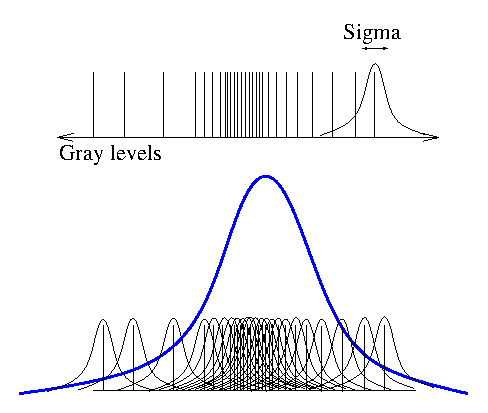
\includegraphics[width=0.48\textwidth]{ParzenWindowing13.eps}}

In a typical registration problem, direct access to the marginal 
and joint probability densities is not available and hence the
densities must be estimated from the image data. Parzen windows 
(also known as kernel density estimators) can be used for this purpose.
In this scheme, the densities are constructed by taking intensity 
samples $S$ from the image and super-positioning kernel functions 
$K(\cdot)$ centered on the elements of $S$ as illustrated in
Figure \ref{fig:ParzenWindowing}:

A variety of functions can be used as the smoothing kernel with the
requirement that they are smooth, symmetric, have zero mean and
integrate to one. For example, boxcar, Gaussian and B-spline functions are
suitable candidates.  A smoothing parameter is used to scale the kernel
function.  The larger the smoothing parameter, the wider the kernel function
used and hence the smoother the density estimate. If the parameter is too
large, features such as modes in the density will get smoothed out.  On the
other hand, if the smoothing parameter is too small, the resulting density
may be too noisy. The estimation is given by the following equation.

\begin{equation}
p(a) \approx P^{*}(a) = \frac{1}{N} \sum_{s_j \in S} K\left(a - s_j\right)
\end{equation}

Choosing the optimal smoothing parameter is a difficult research problem and
beyond the scope of this software guide.  Typically, the optimal value of the
smoothing parameter will depend on the data and the number of samples used.

\subsubsection{Viola and Wells Implementation}

The Insight Toolkit has two mutual information metric implementations. The
first is \doxygen{MutualInformationImageToImageMetric} and follows the method
specified by Viola and Wells in \cite{Viola1997}.

\index{itk::Mutual\-Information\-Image\-To\-Image\-Metric}

In this implementation, two separate intensity samples $S$ and $R$ are drawn
from the image: the first to compute the density, and the second to approximate
the entropy as a sample mean:
\begin{equation}
H(A) = \frac{1}{N} \sum_{r_j \in R} \log P^{*}(r_j).
\end{equation}
Gaussian density is used as a smoothing kernel, where the standard deviation
$\sigma$ acts as the smoothing parameter.

\index{itk::Mutual\-Information\-Image\-To\-Image\-Metric!SetNumberOfSpatialSamples()}

The number of spatial samples used for computation is defined using
the \code{SetNumberOfSpatialSamples()} method. Typical values range from 50 to 100.
Note that computation involves an $N \times N$ loop and hence, the computation
burden becomes very expensive when a large number of samples is used.

\index{itk::Mutual\-Information\-Image\-To\-Image\-Metric!SetFixedImageStandardDeviation()}
\index{itk::Mutual\-Information\-Image\-To\-Image\-Metric!SetMovingImageStandardDeviation()}
The quality of the density estimates depends on the choice of the standard
deviation of the Gaussian kernel. The optimal choice will depend on the
content of the images.  In our experience with the toolkit, we have found
that a standard deviation of 0.4 works well for images that have been
normalized to have a mean of zero and standard deviation of 1.0. The standard
deviation of the fixed image and moving image kernel can be set separately
using methods
\code{SetFixedImageStandardDeviation()} and \code{SetMovingImageStandardDeviation()}.

\subsubsection{Mattes et al. Implementation}
The second form of mutual information metric available in ITK follows the
method specified by Mattes et al. in \cite{Mattes2001} and is implemented by
the \doxygen{MattesMutualInformationImageToImageMetric} class.

\index{itk::Mattes\-Mutual\-Information\-Image\-To\-Image\-Metric}
In this implementation, only one set of intensity samples is drawn from the
image.  Using this set, the marginal and joint probability density function
(PDF) is evaluated at discrete positions or bins uniformly spread within the
dynamic range of the images. Entropy values are then computed by summing over
the bins.

\index{itk::Mattes\-Mutual\-Information\-Image\-To\-Image\-Metric!SetNumberOfSpatialSamples()}
\index{itk::Mattes\-Mutual\-Information\-Image\-To\-Image\-Metric!SetNumberOfHistogramBins()}

The number of spatial samples used is set using method 
\code{SetNumberOfSpatialSamples()}. The number of bins used to compute
the entropy values is set via \code{SetNumberOfHistogramBins()}.

Since the fixed image PDF does not contribute to the metric derivatives, it
does not need to be smooth. Hence, a zero order (boxcar) B-spline kernel is
used for computing the PDF. On the other hand, to ensure smoothness, a third
order B-spline kernel is used to compute the moving image intensity PDF. The
advantage of using a B-spline kernel over a Gaussian kernel is that the
B-spline kernel has a finite support region. This is computationally
attractive, as each intensity sample only affects a small number of bins and
hence does not require a $N \times N$ loop to compute the metric value.

During the PDF calculations, the image intensity values are linearly scaled
to have a minimum of zero and maximum of one. This rescaling means that a
fixed B-spline kernel bandwidth of one can be used to handle image data with
arbitrary magnitude and dynamic range.


\subsection{Kullback-Leibler distance metric}
Another information based metric is the \doxygen{KullbackLeiblerCompareHistogramImageToImageMetric} metric. Kullback-Leibler distance measures the relative entropy between two discrete 
probability distributions. The distributions are obtained from the histograms of the two 
input images, $A$ and $B$. 

The Kullback-Liebler distance between two histograms is given by
\begin{equation}
KL(A,B) =  \sum_i^N p_A(i) \times \log \frac{ p_A(i) }{p_B(i) }
\end{equation}

The distance is always non-negative and is zero only if the two distributions 
are the same. Note that the distance is not symmetric. In other 
words, $KL(A,B) \neq KL(B,A)$. Nevertheless, if the distributions are not too dissimilar, 
the difference betwween $KL(A,B)$ and $KL(B,A)$ is small.

The implementation in ITK is based on \cite{Chung2002}

\subsection{Normalized Mutual Information Metric}
Given two images, $A$ and $B$, the normalized mutual information may be computed as 
\begin{equation}
NMI(A,B) = 1 + \frac{I(A,B)}{H(A,B)} = \frac{H(A) + H(B)}{H(A,B)}
\end{equation}
where the entropy of the images, $H(A)$, $H(B)$, the mutual 
inoformation, $I(A,B)$ and the joint entropy $H(A,B)$ are computed as mentioned 
in \ref{sec:MutualInformationMetric}. Details of the implementation may be found in 
the \cite{Hajnal2001}.

\subsection{Cardinality Match Metric}
\index{itk::Match\-Cardinality\-Image\-To\-Image\-Metric}
The \doxygen{MatchCardinalityImageToImageMetric} computes cardinality of the set of pixels 
that match exactly between the moving and fixed images. In other words, it computes the 
number of pixel matches and mismatches between the two images. The match is designed for 
label maps. All pixel mismatches are considered equal whether they are between label 1 
and label 2 or between label 1 and label 500. In other words, the magnitude of an 
individual label mismatch is not relevant, or the occurence of a label mismatch 
is important. 

The spatial correspondance between the fixed and moving images is established using 
a \doxygen{Transform} using the \code{SetTransform()} method and an interpolator 
using \code{SetInterpolator()}. Given that we are matching pixels with labels, 
it is advisable to use Nearest Neighbor interpolation.

\subsection{Kappa Statistics Metric}
\index{itk::Kappa\-Statistic\-Image\-To\-Image\-Metric}
The \doxygen{KappaStatisticImageToImageMetric} computes spatial intersection of 
two binary images. The metric here is designed for matching pixels in two images 
with the same exact value, which may be set using \code{SetForegroundValue()}. 
Given two images $A$ and $B$, the $\kappa$ coefficient is computed as
 
\begin{equation}
\kappa = \frac{|A| \cap |B|}{|A| + |B|}
\end{equation}

This computes the fraction of area in the two images that is common to both 
the images. In the computation of the metric, only foreground pixels are considered.

\subsection{Gradient Difference Metric}
\index{it::Gradient\-Difference\-Image\-To\-Image\-Metric}
This \doxygen{GradientDifferenceImageToImageMetric} metric evaluates the 
difference in the derivatives of the moving and fixed images. and adds 
them after passing them through a function $\frac{1}{1+x}$.



\fi

% the clearpage command helps to avoid orphans in the title of the next
% section.
\clearpage

\section{Optimizers}
\label{sec:Optimizers}
\ifitkFullVersion

\index{itk::Optimizer|textbf}
\index{itk::SingleValuedNonLinearOptimizer|textbf}


\begin{figure}
\center
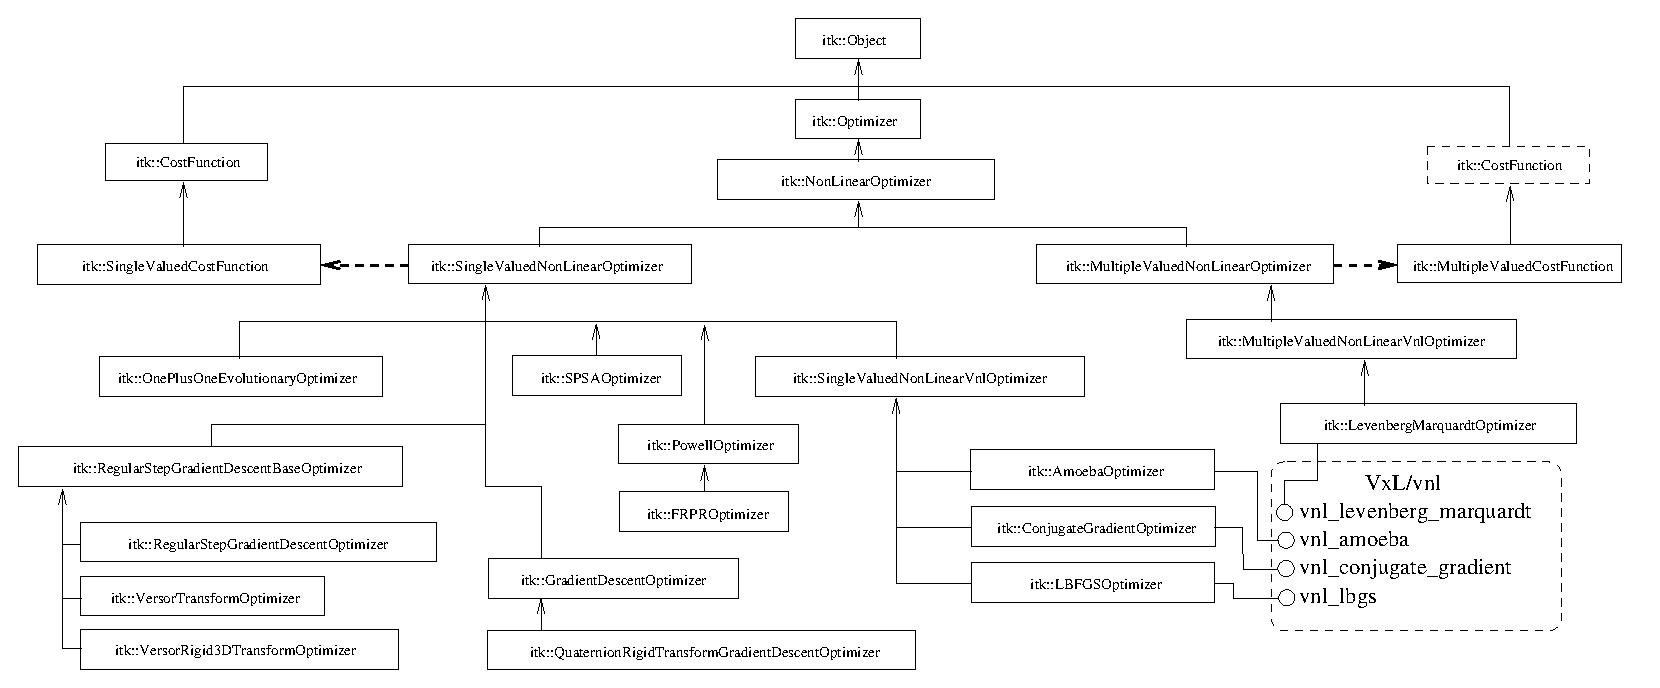
\includegraphics[width=16cm]{OptimizersHierarchy.eps}
\itkcaption{Class diagram of the Optimizers hierarchy.}
\label{fig:OptimizersHierarchy}
\end{figure}

Optimization algorithms are encapsulated as \code{itk::Optimizer} objects
within ITK. Optimizers are generic and can be used for applications other than
registration.  Within the registration framework,
\code{itk::SingleValuedNonLinearOptimizer} are used to optimize the metric
criterion with respect to the transform parameters.

\index{itk::Optimizer!SetInitialPosition()}
\index{itk::Optimizer!StartOptimization()}
\index{itk::Optimizer!GetCurrentPosition()}

The basic input to an optimizer is a cost function object. In the context
of registration, \code{itk::ImageToImageMetric} provide this functionality.
The initial parameters are set using \code{SetInitialPosition()} and
the optimization algorithm is invoked by \code{StartOptimization()}.
Once the optimization has finished, the final parameters can be obtained
using \code{GetCurrentPosition()}.

\index{itk::Optimizer!SetScales()}
Some optimizers also allows rescaling of the individual parameters. This
is convenient for normalizing parameters spaces where some parameters
have different dynamic ranges. For example, the first parameter of
\code{Euler2DTransform} represent an angle while the last two parameters
the translation. A unit change in angle has a much greater impact on
an image than a unit change in translation. This difference in scale appears
as long narrow valleys in the search space making the optimization problem
diffcult. Rescaling the translation parameters can help to fix this problem.
Scales are represented as \code{Array} of doubles and set defined using
\code{SetScales()}.

The types of \code{itk::SingleValuedNonLinearOptimizer} currently available
in ITK are:

\index{itk::AmoebOptimizer|textbf}
\index{itk::ConjugateGradientOptimizer|textbf}
\index{itk::GradientDescentOptimizer|textbf}
\index{itk::QuaternionRigidTransformGradientDescentOptimizer|textbf}
\index{itk::LBFGSOptimizer|textbf}
\index{itk::OnePlusOneEvolutionaryOptimizer|textbf}
\index{itk::RegularStepGradientDescentOptimizer|textbf}
\index{itk::VersorTransformOptimizer|textbf}
\index{itk::LevenbergMarquardtOptimizer|textbf}

\begin{itemize}

\item \textbf{Amoeba}: Nelder-Meade downhill simplex.  This optimizer is
actually implemented in the \code{VxL/vnl} numerics toolkit.  The ITK class
\code{itk::AmoebaOptimizer} is merely an adaptor class.

\item \textbf{Conjugate Gradient}: Fletcher-Reeves form 
of conjugate gradient with or without preconditioning. Also an adaptor to an
optimizer in \code{vnl}.

\item \textbf{Gradient Descent}: Advance parameters in the direction of the
gradient where the step size is governed by a learning rate. 

\item \textbf{Quaternion Rigid Transform Gradient Descent}: 
A specialized version of \code{GradientDescentOptimizer} for
\code{QuaternionRigidTransform} parameters, where the parameters representing
the quaternion is normalize to a magnitude to one at each iteration to
represent a pure rotation.

\item \textbf{LBFGS}: Limited memory Broyden, Fletcher, Goldfarb
and Shannon minmization. It is an adaptor to an optimizer in \code{vnl}.

\item \textbf{One Plus One Evolutionary}: Strategy that simulates the
biological evolution of a set of samples in the search space. This optimizer
is mainly used in the process of bias correction for MRI images.

\item \textbf{Regular Step Gradient Descent}: Advance parameters in the
direction of the gradient where a bipartition scheme is used to compute
the step size. 

\item \textbf{Versor Transform Optimizer}: A specialized version of
\code{RegularStepGradientDescentOptimizer} for \code{VersorTransform}
parameters  where the current rotation is composed with the gradient rotation
to produce the new rotation vector. It follows the definition of versor
gradients defined by Hamilton~\cite{Hamilton1866}.

\end{itemize}

A parallel hierarchy exists for optimizing multiple-valued cost functions. The
base optimizer in this branch of the hierarchy is the
\code{itk::MultipleValuedNonLinearOptimizer} whose only current derived class
is:

\begin{itemize}

\item \textbf{Levenberg Marquardt}: Non-linear least squares minimization.
Adapted to an optimizer in \code{vnl}.

\end{itemize}


Figure \ref{fig:OptimizersHierarchy} illustrates the full class hierarchy of
optimizers in ITK. Optimizers in the lower right corner are adaptors classes to
optimizers existing in the \code{VxL/vnl} numerics toolkit. The optimizers
interact with the \code{itk::CostFunction} class. In the registration framework
this cost function is reimplemented in the form of \code{itk::ImageToImageMetric}.






\fi



\subsection{Registration using Match Cardinality metric}
\label{sec:RegistrationMatchCardinality}
\ifitkFullVersion
\input{ImageRegistration10.tex}
\fi


\subsection{Registration using the One plus One Evolutionary Optimizer}
\label{sec:RegistrationOnePlusOne}
\ifitkFullVersion
\input{ImageRegistration11.tex}
\fi



\subsection{Registration using masks constructed with Spatial objects}
\label{sec:RegistrationSpatialObjects}
\ifitkFullVersion
\input{ImageRegistration12.tex}
\fi



\subsection{Rigid registrations incorporating prior knowledge}
\label{sec:RegistrationCentered2DTransform}
\ifitkFullVersion
\input{ImageRegistration13.tex}
\fi
% the clearpage command helps to avoid orphans in the title of the next
% section.
\clearpage

\section{Image Pyramids}
\label{sec:ImagePyramids}
\ifitkFullVersion

\index{itk::Multi\-Resolution\-Pyramid\-Image\-Filter}

In ITK, the \doxygen{MultiResolutionPyramidImageFilter} can be used to create
a sequence of reduced resolution images from the input image.  The
down-sampling is performed according to a user defined multi-resolution
schedule. The schedule is specified as an \doxygen{Array2D} of integers,
containing shrink factors for each multi-resolution level (rows) for each
dimension (columns). For example,

\small
\begin{verbatim}
8 4 4
4 4 2
\end{verbatim}
\normalsize

is a schedule for a three dimensional image for two multi-resolution levels.
In the first (coarsest) level, the image is reduced by a factor of 8
in the column dimension, factor of 4 in the row dimension and a factor
of 4 in the slice dimension. In the second level, the image reduced
by a factor of 4 in the column dimension, 4 in the row dimension and
2 in the slice dimension.

\index{itk::Multi\-Resolution\-Pyramid\-Image\-Filter!SetNumberOfLevels()}

The method \code{SetNumberOfLevels()} is used to set the number of
resolution levels in the pyramid. This method will allocate memory
for the schedule and generate a default table with the starting
(coarsest) shrink factors for all dimensions set to $2^(M-1)$,
where $M$ is the number of levels. All factors are halved for
all subsequent levels. For example, if we set the number of levels
to 4, the default schedule is then:

\small
\begin{verbatim}
8 8 8
4 4 4
2 2 2
1 1 1
\end{verbatim}
\normalsize

\index{itk::Multi\-Resolution\-Pyramid\-Image\-Filter!GetSchedule()}
\index{itk::Multi\-Resolution\-Pyramid\-Image\-Filter!SetSchedule()}
\index{itk::Multi\-Resolution\-Pyramid\-Image\-Filter!SetStartingShrinkFactors()}

The user can get a copy of the schedule using method \code{GetSchedule()},
make modifications, and reset it using method \code{SetSchedule()}.
Alternatively, a user can create a default table by specifying the
starting (coarsest) shrink factors using the method
\code{SetStartingShrinkFactors()}. The factors for the subsequent
levels are generated by halving the factor or setting it to one,
depending on which is larger. For example, for a 4 level pyramid
and starting factors of 8, 8 and 4, the generated schedule would be:

\small
\begin{verbatim}
8 8 4
4 4 2
2 2 1
1 1 1
\end{verbatim}
\normalsize

When this filter is triggered by \code{Update()}, $M$ outputs are produced
where the $m$-th output corresponds to the $m$-th level of the pyramid.
To generate these images, Gaussian smoothing is first performed using a
\doxygen{DiscreteGaussianImageFilter} with the variance set to $(s/2)^2$,
where $s$ is the shrink factor. The smoothed images are then sub-sampled using
a \doxygen{ShrinkImageFilter}.

\fi


% the clearpage command helps to avoid orphans in the title of the next
% section.
\clearpage

\section{Deformable Registration}
\label{sec:DeformableRegistration}
\ifitkFullVersion
%%%%%%%%%%%%%%%%%%%%%%%%%%%%%%%%%%%%%%%%%%%%%%%%%%%%%%%%%%%%%%%
%
%
%   This file is included in Registration.tex
%
%   Labels and section entries are defined in that file.
%
%
%
%%%%%%%%%%%%%%%%%%%%%%%%%%%%%%%%%%%%%%%%%%%%%%%%%%%%%%%%%%%%%%%


\subsection{FEM-Based Image Registration}
\label{sec:FEMBasedImageRegistration}

\begin{figure}
\centering
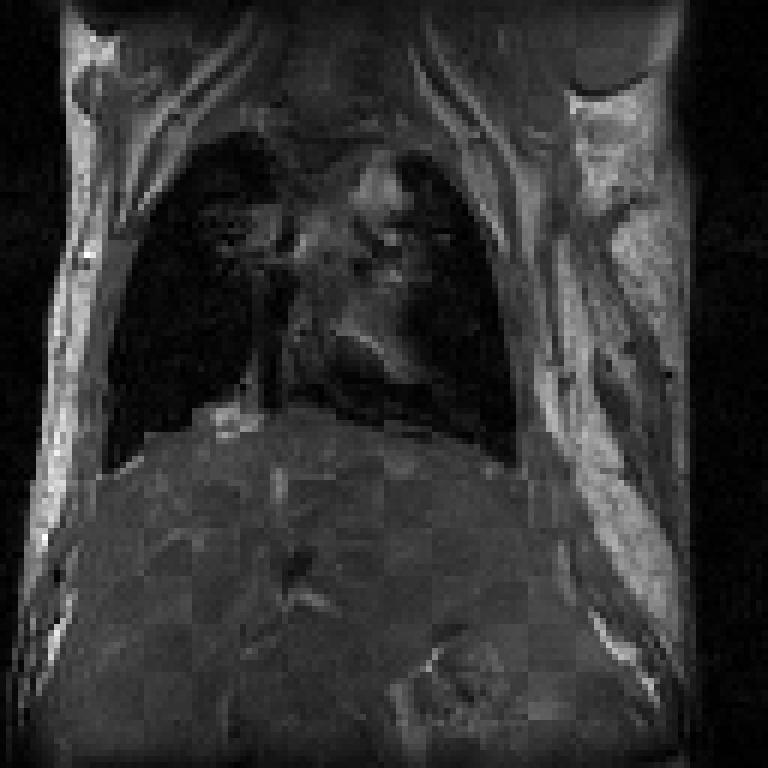
\includegraphics[width=0.44\textwidth]{DeformableRegistration1CheckerboardBefore.eps}
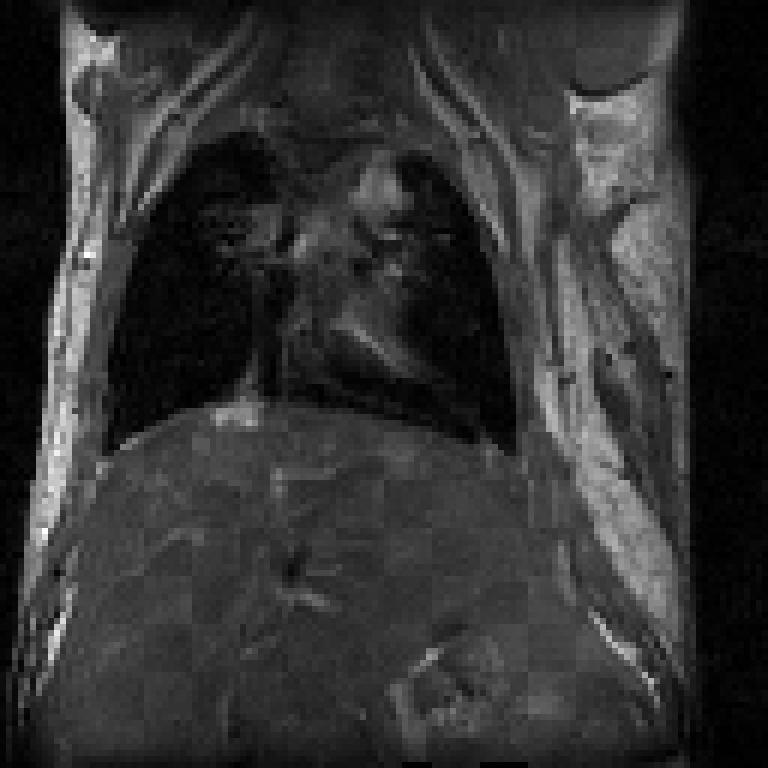
\includegraphics[width=0.44\textwidth]{DeformableRegistration1CheckerboardAfter.eps}
\itkcaption[FEM-based deformable registration results]{Checkerboard comparisons
before and after FEM-based deformable registration.}
\label{fig:DeformableRegistration1Output}
\end{figure}

\input{DeformableRegistration1.tex}

Figure \ref{fig:DeformableRegistration1Output} presents the results of
the FEM-based deformable registration applied to two time-separated
slices of a living rat dataset.  Checkerboard comparisons of the two
images are shown before registration (left) and after registration
(right).  Both images were acquired from the same living rat, the
first after inspiration of air into the lungs and the second after
exhalation.  Deformation occurs due to the relaxation of the diaphragm
and the intercostal muscles, both of which exert force on the lung tissue
and cause air to be expelled.

The following is a documented sample parameter file that can be used with this
deformable registration example.  This example demonstrates the setup of a
basic registration problem that does not use multi-resolution strategies.  As a
result, only one value for the parameters between \texttt{(\# of pixels per
element)} and \texttt{(maximum iterations)} is necessary.  In order to use a
multi-resolution strategy, you would have to specify values for those
parameters at each level of the pyramid.

\small
\verbatiminput{FiniteElementRegistrationParameters1.txt}
\normalsize

\subsection{BSplines Image Registration}
\label{sec:BSplinesImageRegistration}
\input{DeformableRegistration4.tex}


\subsection{Level Set Motion for Deformable Registration}
\label{sec:LevelSetMotionForDeformableRegistration}
\input{DeformableRegistration5.tex}


\subsection{BSplines Multi-Grid Image Registration}
\label{sec:BSplinesMultiGridImageRegistration}
\input{DeformableRegistration6.tex}


\subsection{BSplines Multi-Grid Image Registration in 3D}
\label{sec:BSplinesMultiGridImageRegistrationIn3D}
\input{DeformableRegistration7.tex}


\subsection{Image Warping with Kernel Splines}
\label{sec:ImageWarpingWithKernelSplines}
\input{LandmarkWarping2.tex}


\subsection{Image Warping with BSplines}
\label{sec:ImageWarpingWithBSplines}
\input{BSplineWarping1.tex}

\fi

% the clearpage command helps to avoid orphans in the title of the next
% section.
\clearpage

\section{Demons Deformable Registration}
\label{sec:DemonsDeformableRegistration}
\ifitkFullVersion
%%%%%%%%%%%%%%%%%%%%%%%%%%%%%%%%%%%%%%%%%%%%%%%%%%%%%%%%%%%%%%%
%
%
%   This file is included in Registration.tex
%
%   Lablels and section entries are defined in that file.
%
%
%
%%%%%%%%%%%%%%%%%%%%%%%%%%%%%%%%%%%%%%%%%%%%%%%%%%%%%%%%%%%%%%%

For the problem of intra-modality deformable registration, the Insight
Toolkit provides an implementation of Thirion's ``demons'' algorithm
\cite{Thirion1995b,Thirion1998}. 
In this implementation, each image is viewed as a set of iso-intensity
contours.  The main idea is that a regular grid of forces deform an image by
pushing the contours in the normal direction.  The orientation and magnitude
of the displacement is derived from the instantaneous optical flow equation:

\begin{equation}
\bf{D}(\bf{X}) \cdot \nabla f(\bf{X}) = - \left(m(\bf{X}) - f(\bf{X}) \right)
\label{eqn:OpticalFlow}
\end{equation}

In the above equation, $f(\bf{X})$ is the fixed image, $m(\bf{X})$
is the moving image to be registered, and $\bf{D}(\bf{X})$ is the displacement 
or optical flow between the images. It is well known in optical flow
literature that Equation \ref{eqn:OpticalFlow} is insufficient to specify 
$\bf{D}(\bf{X})$ locally and is usually determined using some form of
regularization. For registration, the projection of the vector on the
direction of the intensity gradient is used:

\begin{equation}
\bf{D}(\bf{X}) = - \frac
{\left(  m(\bf{X}) - f(\bf{X}) \right) \nabla f(\bf{X})}
{\left\|  \nabla f \right\|^2 } 
\end{equation}

However, this equation becomes unstable for small values of the image gradient,
resulting in large displacement values. To overcome this problem, Thirion
re-normalizes the equation such that:

\begin{equation}
\bf{D}(\bf{X}) = - \frac
{\left(  m(\bf{X}) - f(\bf{X}) \right) \nabla f(\bf{X})}
{\left\|  \nabla f \right\|^2 + \left(  m(\bf{X}) - f(\bf{X}) \right)^2 / K } 
\label{eqn:DemonsDisplacement}
\end{equation}

Where $K$ is a normalization factor that accounts for the units imbalance
between intensities and gradients. This factor is computed as the mean squared
value of the pixel spacings. The inclusion of $K$ make the force computation to
be invariant to the pixel scaling of the images.

Starting with an initial deformatin field $\bf{D}^{0}(\bf{X})$, the demons
algorithm iteratively updates the field using Equation
\ref{eqn:DemonsDisplacement} such that the field at the $N$-th iteration is
given by:

\begin{equation}
\bf{D}^{N}(\bf{X}) = \bf{D}^{N-1}(\bf{X}) - \frac
{\left(  m(\bf{X}+ \bf{D}^{N-1}(\bf{X})) 
- f(\bf{X}) \right) \nabla f(\bf{X})}
{\left\|  \nabla f \right\|^2 + \left(  
m(\bf{X}+ \bf{D}^{N-1}(\bf{X}) )
 - f(\bf{X}) \right)^2 } 
\label{eqn:DemonsUpdateEquation}
\end{equation}

Reconstruction of the deformation field is an ill-posed problem where
matching the fixed and moving images has many solutions. For example, since
each image pixel is free to move independently, it is possible that all
pixels of one particular value in $m(\bf{X})$ could map to a single image
pixel in $f(\bf{X})$ of the same value. The resulting deformation field may
be unrealistic for real-world applications. An option to solve for the field
uniquely is to enforce an elastic-like behavior, smoothing the deformation
field with a Gaussian filter between iterations.

In ITK, the demons algorithm is implemented as part of the finite difference
solver (FDS) framework and its use is demonstrated in the following example.

\input{DeformableRegistration2.tex} 

A variant of the force computation is also implemented in which the gradient of
the deformed moving image is also involved. This provides a level of symmetry
in the force calculation during one iteration of the PDE update. The equation
used in this case is

\begin{equation}
\bf{D}(\bf{X}) = - \frac
{2 \left(  m(\bf{X}) - f(\bf{X}) \right) \left(  \nabla f(\bf{X}) +  \nabla g(\bf{X}) \right) }
{\left\|  \nabla f + \nabla g \right\|^2 + \left(  m(\bf{X}) - f(\bf{X}) \right)^2 / K } 
\label{eqn:DemonsDisplacement}
\end{equation}

The following example illustrates the use of this defomable registration
method.

\input{DeformableRegistration3.tex} 




\fi

\section{Visualizing Deformation fields}
\label{sec:VisualizingDeformationFields}
\ifitkFullVersion
%%%%%%%%%%%%%%%%%%%%%%%%%%%%%%%%%%%%%%%%%%%%%%%%%%%%%%%%%%%%%%%
%
%
%   This file is included in Registration.tex
%
%   Lablels and section entries are defined in that file.
%
%
%
%%%%%%%%%%%%%%%%%%%%%%%%%%%%%%%%%%%%%%%%%%%%%%%%%%%%%%%%%%%%%%
Vector deformation fields may be visualized using Paraview.
Paraview \cite{ParaviewBook} is an open-source, multi-platform visualization application and uses the Visualization Toolkit as the data processing and rendering engine and has a user interface written using a unique blend of Tcl/Tk and C++. You may download it from http://paraview.org.

\subsection{Visualizing 2D deformation fields}
Let us visualize the deformation field obtained from Demons Registration algorithm generated from Insight/Examples/Registration/DeformableRegistration2.cxx.

Load the Deformation field in Paraview. (The deformation field must be capable of handling vector data, such as MetaImages). Paraview shows a color map of the magnitudes of the deformation fields as shown in \ref{fig:ParaviewScreenshot1}.

Covert the deformation field to 3D vector data using a {\it Calculator}. The Calculator may be found in the {\it Filter} pull dowm menu. A screenshot of the calculator tab is shown in Figure \ref{fig:ParaviewScreenshot2}. Although the deformation field is a 2D vector, we will generate a 3D vector with the third component set to 0 since Paraview generates glyphs only for 3D vectors. You may now apply a glyph of arrows to the resulting 3D vector field by using {\it Glyph} on the menu bar. The glphs obtained will be very dense since a glyph is generated for each point in the data set. To better visualize the deformation field, you may adopt one of the following approaches. 

Reduce the number of glyphs by reducing the number in {\it Max. Number of Glyphs} to reasonable amount. This uniformly downsamples the number of glyphs. Alternatively, you may apply a {\it Threshold} filter to the {\it Magnitude} of the vector dataset and then glyph the vector data that lies above the threshold. This eliminates the smaller deformation fields that clutter the display. You may now reduce the number of glyphs to a reasonable value.

Figure \ref{fig:ParaviewScreenshot3} shows the vector field visualized using Paraview by thresholding the vector magnitudes by 2.1 and restricting the number of glyphs to 100.

\begin{figure}
\center
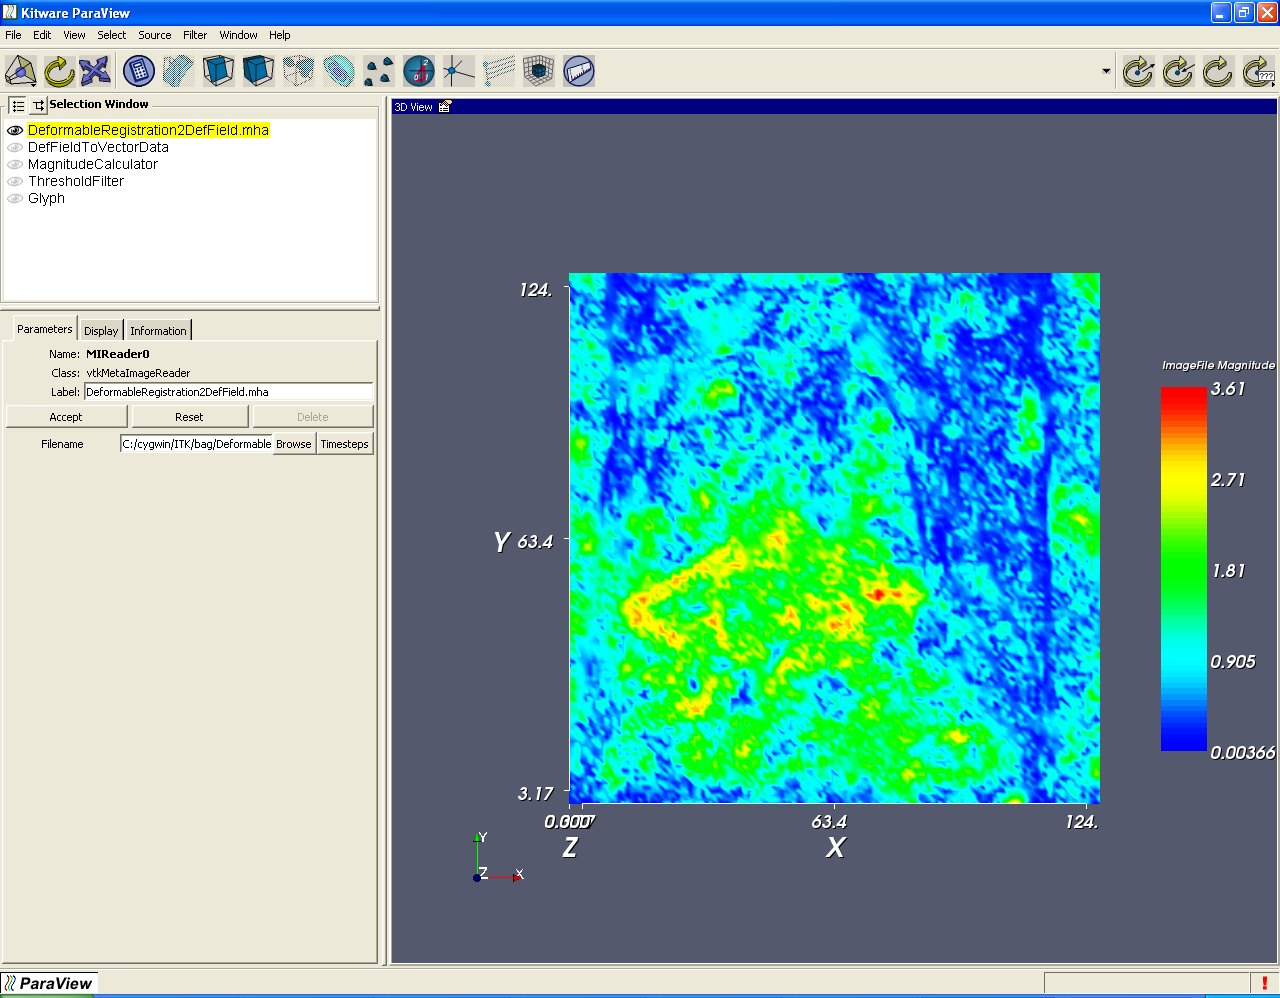
\includegraphics[width=\textwidth]{ParaviewScreenshot1.eps}
\itkcaption[Deformation field magnitudes]{Deformation field magnitudes displayed using Paraview}
\label{fig:ParaviewScreenshot1}
\end{figure}

\begin{figure}
\center
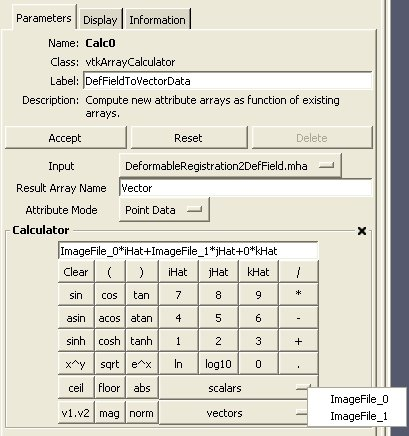
\includegraphics[width=0.3\textwidth]{ParaviewScreenshot2.eps}
\itkcaption[Calculator]{Calculators and filters may be used to compute the vector magnitude, compose vectors etc.}
\label{fig:ParaviewScreenshot2}
\end{figure}

\begin{figure}
\center
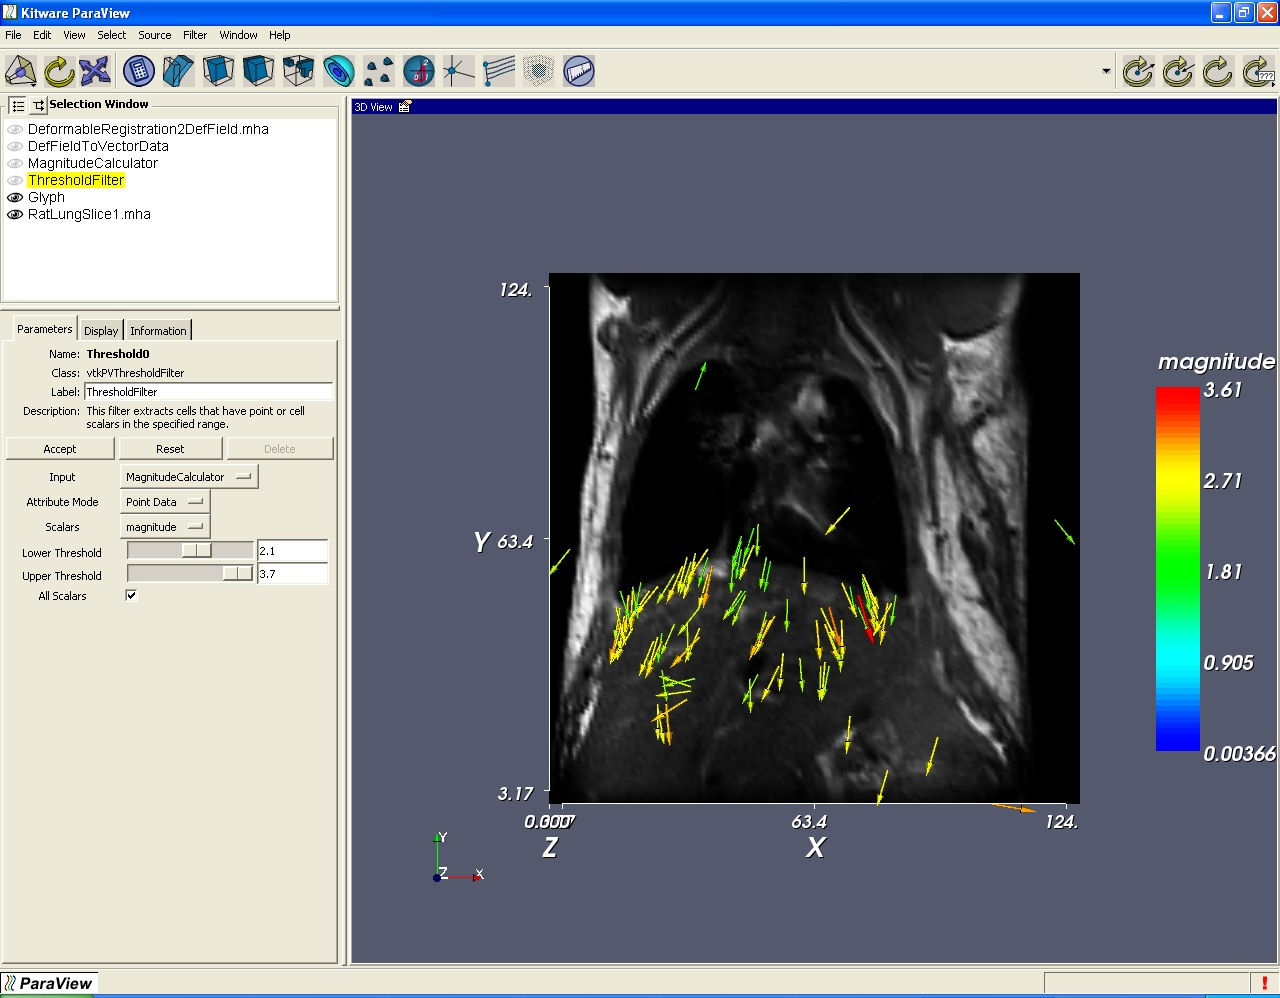
\includegraphics[width=\textwidth]{ParaviewScreenshot3.eps}
\itkcaption[Visualized Def field]{Deformation field visualized using Paraview after thresholding and subsampling.}
\label{fig:ParaviewScreenshot3}
\end{figure}



\subsection{Visualizing 3D deformation fields}
Let us create a 3D deformation field. We will use Thin Plate Splines to warp a 3D dataset and create a deformation field. We will pick a set of point landmarks and translate them to provide a specification of correspondences at point landmarks. Note that the landmarks have been picked randomly for purposes of illustration and are not intended to portray a true deformation. The landmarks may be used to produce a deformation field in several ways. Most techniques minimize some regularizing functional representing the irregularity of the deformation field, which is usually some function of the spatial derivatives of the field. Here will we use {\it thin plate splines}. Thin plate splines minimize the regularizing functional 

\begin{equation}
I[f(x,y)] = \iint (f^2_{xx} + 2 f^2_{xy} + f^2_{yy}) dx dy
\end{equation}
where the subscripts denote partial derivatives of f.

The code for this section can be found in Insight/Examples/Registration/ThinPlateSplineWarp.cxx

We may now proceed as before to visualize the deformation field using Paraview as shown in Figure \ref{fig:ParaviewScreenshot4}.

\begin{figure}
\center
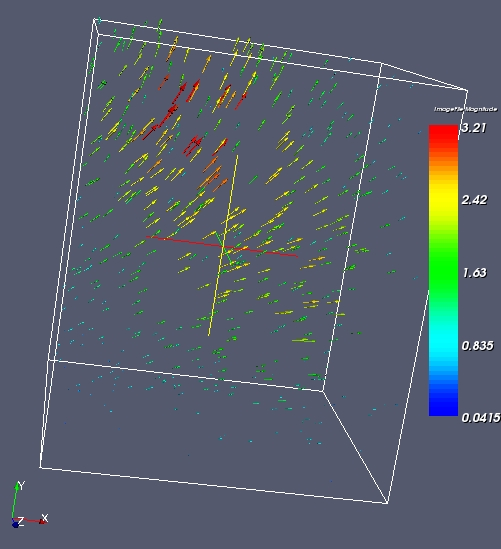
\includegraphics[width=0.7\textwidth]{ParaviewScreenshot4.eps}
\itkcaption[Visualized Def field4]{3D Deformation field visualized using Paraview.}
\label{fig:ParaviewScreenshot4}
\end{figure}




\fi

\ifitkFullVersion
%%%%%%%%%%%%%%%%%%%%%%%%%%%%%%%%%%%%%%%%%%%%%%%%%%%%%%%%%%%%%%%
%
%
%   This file is included in DeformableRegistration.tex
%
%   Labels and section entries are defined in that file.
%
%
%
%%%%%%%%%%%%%%%%%%%%%%%%%%%%%%%%%%%%%%%%%%%%%%%%%%%%%%%%%%%%%%
Let us register the deformed volumes generated by Thin plate warping in the
previous example using DeformableRegistration4.cxx. Since ITK is in general
N-dimensional, the only change in the example is to replace the
\code{ImageDimension} by 3.

The registration method uses B-splines and an LBFGS optimizer. The trace in
Table. \ref{tab:LBFGStrace} prints the trace of the optimizer through the
search space.

\begin{table}
\begin{center}
\begin{tabular}{\tableconfiguration}
\hline
\textbf{Iteration} &
\textbf{Function value} &
\textbf{$\|G\|$} &
\textbf{Step length} \\
\hline\hline
   1    &        156.981  &    14.911  & 0.202 \\
   2    &        68.956    &    11.774    &    1.500 \\
   3    &        38.146    &    4.802     &   1.500 \\
   4    &        26.690    &    2.515     &   1.500 \\
   5    &        23.295    &    1.106     &   1.500\\
   6    &        21.454    &    1.032     &   1.500\\
   7    &        20.322    &    1.557     &   1.500\\
   8    &        19.751    &    0.594     &   1.500\\
\hline
\end{tabular}
\end{center}
\itkcaption[LBFGS Optimizer trace]{LBFGS Optimizer trace.
\label{tab:LBFGStrace}}
\end{table}

Here $\|G\|$ is the norm of the gradient at the current estimate of the
minimum, $x$. ``Function Value" is the current value of the function, f(x).

The resulting deformation field that maps the moving to the fixed image is
shown in \ref{fig:DeformationFieldOutput}. A difference image of two slices
before and after registration is shown in
\ref{fig:DefRegistrationDiffScreenshot}. As can be seen from the figures, the
deformation field is in close agreement to the one generated from the Thin
plate spline warping.

\begin{figure}
\center
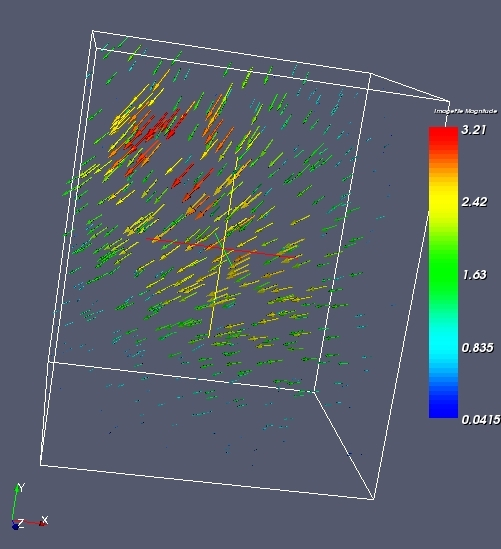
\includegraphics[width=0.6\textwidth]{ParaviewScreenshot5.eps}
\itkcaption[Deformation field output]{Resulting deformation field that maps the moving image to the fixed image.}
\label{fig:DeformationFieldOutput}
\end{figure}

\begin{figure}
\center
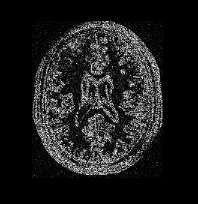
\includegraphics[width=0.44\textwidth]{DeformableRegistration4DiffBefore.eps}
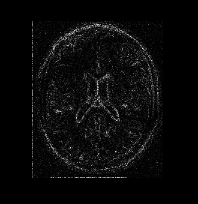
\includegraphics[width=0.44\textwidth]{DeformableRegistration4DiffAfter.eps}
\itkcaption[Difference image]{Difference image from a slice before and after registration.}
\label{fig:DefRegistrationDiffScreenshot}
\end{figure}



\fi


% the clearpage command helps to avoid orphans in the title of the next
% section.
\clearpage

\section{Model Based Registration}
\label{sec:ModelBasedRegistration}
\ifitkFullVersion
%%%%%%%%%%%%%%%%%%%%%%%%%%%%%%%%%%%%%%%%%%%%%%%%%%%%%%%%%%%%%%%
%
%
%   This file is included in Registration.tex
%
%   Lablels and section entries are defined in that file.
%
%
%
%%%%%%%%%%%%%%%%%%%%%%%%%%%%%%%%%%%%%%%%%%%%%%%%%%%%%%%%%%%%%%%

\itkpiccaption[Model to Image Registration Framework Components]{The basic components of model based registration are an image, a spatial object, a transform, a metric, an interpolator and an optimizer.\label{fig:ModelToImageRegistrationComponentsDiagram}}
\parpic(8cm,6cm)[r]{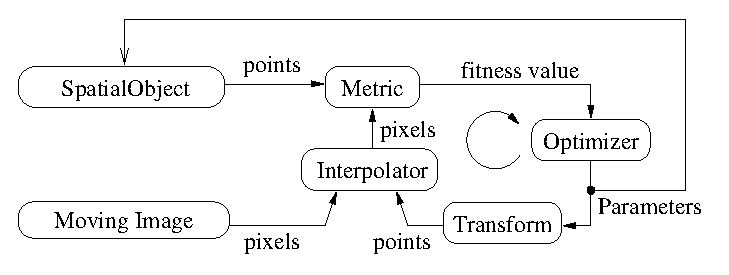
\includegraphics[width=7.5cm]{ModelToImageRegistrationComponentsDiagram.eps}}

This section introduces the concept of registering a geometrical model with an
image. We refer to this concept as \emph{Model Based Registration} but this may
not be the most widespread terminology. In this approach for registration, a
geometrical model is build first and a number of parameters are identified in
the model. Variations of these parameters make possible to adapt the model to
the particular morphology of a specific patient. The task of registration is
then to find the optimal combinations of the model parameters that will make
this model fit as a good representation of the anatomical structure contained
in an image. 


\begin{figure}
\center
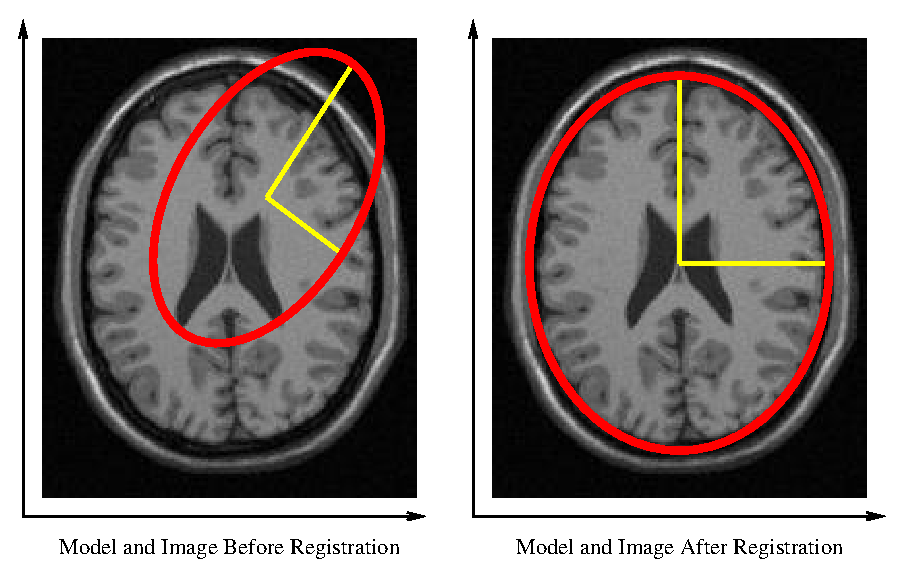
\includegraphics[width=\textwidth]{ModelToImageRegistrationConcept.eps}
\itkcaption[Model to Image Registration Framework Concept]{Basic concept of
  Model-to-Image registration.  A simplified geometrical model (ellipse) is
    registered against an anatomical structure (skull)  by applying a spatial
    transform and modifying the model internal parameters. This image is not
    the result of an actual registration, it is shown here only with the
    purpose of illustrating the concept of model to image registration.}
\label{fig:ModelToImageRegistrationConcept}
\end{figure}


For example, let's say that in the axial view of a brain image we can roughly
approximate the skull with an ellipse. The ellipse becomes our simplified
geometrical model, and registration is the task of finding the best center for
the ellipse, the measures of its axis lengths and its orientation on the plane.
This is illustrated in Figure~\ref{fig:ModelToImageRegistrationConcept}.  If we
compare this aproach with the Image-to-Image registration problem, we can see
that the main difference here is that in addition to mapping the spatial
position of the model, we can also customize internal parameters that change
its shape.

Figure~\ref{fig:ModelToImageRegistrationComponentsDiagram} illustrates the
major components of the registration framework in ITK when a model base
registration problem is configured. The basic input data for the registration
is provided by pixel data in an \doxygen{Image} and by geometrical data stored
in a \doxygen{SpatialObject}. A Metric has to be defined in order to evaluate
the fitness between the model and the image. This fitness value can be improved
by introducing variations in the spatial positioning of the
\doxygen{SpatialObject} and/or by changing its internal parameters. The search
space for the optimizer is now the composition of the transform parameter and
the shape internal parameters.

This same approach can be considered a segmentation technique, since once the
model has been optimally superimposed to the image we could label pixels
according to their associations with specific parts of the model. The
perpectives of model to image registration/segmentation are endless.  Probably
the main advantage of this approach is that, as opposed to image-to-image
registration, it actually provides \emph{Insight} into the anatomical structure
contained in the image. The adapted model becomes a condensed representation of
the essential elements of the anatomical structure.

ITK provides a hierarchy of classes intended to support the construction of
shape models. This hierarchy has the \doxygen{SpatialObject} as its base class.
A number of basic functionalities are defined at this level. For example, the
capacity to evaluate is a given point is \emph{inside} or \emph{outside} of the
model, the capability to form complex shapes by creating hierarchical
conglomerates of basic shapes and the support for basic spatial
parameterizations like scale, orientation and position.

The following sections present examples of the typical uses of these powerful
elements of the toolkit.

%\ifitkFullVersion
\input{ModelToImageRegistration1.tex} 
%\fi





\fi


\section{Point Set Registration}
\label{sec:PointSetRegistration}

The classical algorithm for performing PointSet to PointSet registration is the
Iterative Closest Point (ICP) algorithm.  The following examples illustrate how
this 0 can be used in ITK.

\ifitkFullVersion
\input{IterativeClosestPoint1.tex}
\fi

\ifitkFullVersion
\input{IterativeClosestPoint2.tex}
\fi

\ifitkFullVersion
\input{IterativeClosestPoint3.tex}
\fi


